% !TeX program = lualatex
\documentclass[11pt,a4paper]{article}
\usepackage{szzmaterial}
\usepackage{tikz}
\usetikzlibrary{positioning,arrows.meta,calc,fit,backgrounds,shapes.geometric,shapes.misc,matrix}
\usepackage{pgfplots}
\pgfplotsset{compat=1.18}
\setlist[enumerate]{nosep,leftmargin=2.1em}
\setlist[itemize]{nosep,leftmargin=1.8em}

% --- Box pro algoritmy (pseudokód). Lokální doplněk preambule okruhu. ---
\newtcolorbox{algo}[1][]{enhanced,breakable,colback=teal!4,colframe=teal!55!black,
  boxrule=0.6pt,arc=2pt,left=6pt,right=8pt,top=3pt,bottom=4pt,
  fonttitle=\bfseries,coltitle=white,colbacktitle=teal!55!black,
  title={\faCogs\enspace Algoritmus \textemdash\ #1}}
% Komentář v pseudokódu
\newcommand{\cmt}[1]{\hfill{\footnotesize\itshape\textcolor{black!55}{$\triangleright$ #1}}}

% --- Společné značení grafů a stromů v obrázcích ---
\tikzset{
  vrch/.style={circle,draw=blue!55!black,fill=blue!8,thick,minimum size=7.5mm,inner sep=1pt,font=\small},
  vrchA/.style={circle,draw=red!55!black,fill=red!10,thick,minimum size=7.5mm,inner sep=1pt,font=\small},
  vrchG/.style={circle,draw=green!50!black,fill=green!10,thick,minimum size=7.5mm,inner sep=1pt,font=\small},
  bst/.style={circle,draw=blue!55!black,fill=blue!8,thick,minimum size=7mm,inner sep=1pt,font=\small},
  hrana/.style={thick},
  sip/.style={->,>=Stealth,thick},
}

\szztitul{Algoritmy a datové struktury}{I2}{NTIN060 (ADS 1), NTIN061 (ADS 2)}

\begin{document}
\maketitle
\tableofcontents
\bigskip

\section*{Úvod}
\addcontentsline{toc}{section}{Úvod}

Tento materiál pokrývá okruh \textbf{I2 -- Algoritmy a datové struktury} (předměty NTIN060 \emph{Algoritmy a datové struktury 1} a NTIN061 \emph{Algoritmy a datové struktury 2}). Výklad stojí na jediném, ale úplném zdroji z~MFF UK na úrovni obou kurzů: na učebnici M.~Mareše a T.~Vally \emph{Průvodce labyrintem algoritmů} (2.~vydání, edice CZ.NIC, 2022), kterou přednášející obou předmětů uvádějí jako hlavní studijní text a na kterou se odvolává i~oficiální náčrt řešení státnicových otázek. Značení, hloubka i~konvence (pseudokód, model RAM, asymptotická notace) odpovídají této učebnici.

\noindent\textbf{Role důkazů.} Požadavky okruhu kladou důraz na \emph{porozumění a~konstrukci}: navrhnout nebo odsimulovat algoritmus na konkrétním vstupu, sestavit a~vyřešit rekurentní rovnici, určit asymptotickou složitost, případně dát protipříklad. Pojmenované věty proto uvádíme se zněním, intuicí a~krátkým odvozením tam, kde pomáhá pochopení. Požadavky výslovně uvádějí jedinou větu \emph{bez} důkazu, \textbf{Master theorem (kuchařkovou větu)}: stačí přesné znění, tři případy a~aplikace na rekurenci. Naopak korektnost a~složitost algoritmu typu \emph{rozděl a~panuj} se \emph{odvozuje} (sestavit rekurenci a~vyřešit ji), viz otázka léto~2024. \textbf{Dolní odhad $\Omega(n\log n)$} pro porovnávací třídění je krátký argument přes rozhodovací strom a~uvádíme ho celý (využívá ho otázka jaro~2023).

Do výkladu je zařazeno všech pět reálných otázek SZZ k~okruhu z~let 2022--2025 jako řešené příklady; jsou i~v~samostatném dokumentu \emph{Příklady otázek}. Použité zdroje jsou uvedeny na konci.

\medskip
\noindent\textbf{Značení.} Velikost vstupu značíme $n$ (počet prvků posloupnosti, počet vrcholů grafu apod.), u~grafů navíc $m$ pro počet hran. \emph{Časovou složitost} algoritmu chápeme jako počet elementárních operací modelu RAM v~\emph{nejhorším případě} jako funkci $n$; \emph{prostorovou složitost} jako počet použitých paměťových buněk. Logaritmus bez základu znamená $\log_2$ (na základu nezáleží, liší se jen konstanta-krát). Graf je dvojice $G=(V,E)$, $|V|=n$, $|E|=m$; orientovanou hranu z~$u$ do~$v$ píšeme $uv$. Strom kreslíme kořenem nahoru. \emph{Hloubkou} vrcholu $v$ rozumíme \emph{délku nejdelší cesty z~$v$ dolů do listu} a~značíme ji $h(v)$ (list má $h=0$, prázdný strom $h=-1$); \emph{hloubka stromu} je $h$ jeho kořene. (Pozor na konvenci: tutéž veličinu jinde někdy najdete pod názvem „výška``, kdežto „hloubkou vrcholu`` se občas myslí vzdálenost \emph{od} kořene -- zde vždy měříme cestu \emph{dolů k~listu}.)

% ============================================================
\section{Časová a prostorová složitost, asymptotická notace}

První otázkou u~každého algoritmu je „jak je rychlý a~kolik paměti spotřebuje``. Měřit to vteřinami na konkrétním počítači nedává smysl -- výsledek by závisel na stroji, jazyce i~operačním systému. Proto zavádíme abstraktní míru: počítáme \emph{elementární operace} idealizovaného stroje a~zajímá nás, jak jejich počet \emph{roste} s~velikostí vstupu.

\subsection{Model výpočtu a měření složitosti}

\begin{definice}[Výpočetní model RAM, elementární operace]
\emph{RAM} (Random Access Machine) je idealizovaný počítač s~pamětí tvořenou očíslovanými buňkami, do nichž lze v~konstantním čase číst i~zapisovat podle adresy. \emph{Elementární operací} rozumíme jednu instrukci procesoru: aritmetiku ($+,-,\cdot,/,\bmod$), porovnání, logické a~bitové operace, řízení toku (skok, podmíněný skok) a~přístup do paměti. Každá elementární operace trvá jednu časovou jednotku.
\end{definice}

\begin{intuice}
Konkrétní výběr sady elementárních operací změní dobu výpočtu nejvýše konstanta-krát, a~konstanty stejně zanedbáváme. Proto nezáleží na detailech procesoru; podstatný je jen \emph{řád růstu} počtu operací. (U~čísel s~mnoha ciframi je třeba být opatrný -- pak se počítá s~tzv.\ logaritmickou cenou podle počtu bitů; v~běžných úlohách s~čísly velikosti polynomiální v~$n$ má každá operace cenu konstantní.)
\end{intuice}

\begin{definice}[Časová a prostorová složitost, tři případy]
Nechť algoritmus na vstupu velikosti $n$ provede pro každý konkrétní vstup nějaký počet operací. \emph{Časová složitost v~nejhorším případě} $f(n)$ je \emph{maximum} tohoto počtu přes všechny vstupy velikosti $n$; \emph{v~nejlepším případě} minimum; \emph{v~průměrném případě} aritmetický průměr (resp.\ střední hodnota) přes všechny vstupy velikosti $n$. \emph{Prostorová složitost} je maximální počet paměťových buněk použitých v~jednom okamžiku výpočtu.
\end{definice}

\begin{poznamka}
Není-li řečeno jinak, „složitostí`` myslíme nejhorší případ -- dává záruku „nejhůře tolik a~tolik``. Průměrný případ je užitečný tam, kde se nejhorší případ vyskytuje vzácně (typicky Quicksort, sekce~5).
\end{poznamka}

\begin{poznamka}
\textbf{Měření velikosti dat.} \emph{Velikost vstupu} $n$ udáváme v~přirozené míře dané úlohy -- počet prvků posloupnosti, počet vrcholů a~hran grafu, případně \emph{počet bitů} (číslic) zápisu čísla. Volba míry je podstatná: u~číselných úloh se velikost měří \emph{délkou zápisu}, nikoli hodnotou čísla. Jinak bychom dostali klamně příznivé odhady -- např.\ „vyzkoušet všechny dělitele do~$x$`` vypadá jako $O(x)$, ale vůči počtu číslic $\approx\log_{10}x$ je to \emph{exponenciální} (viz příklad o~rozkladu čísla v~sekci~2).
\end{poznamka}

\subsection{Asymptotická notace}

Přesný počet operací (např.\ $2n^2+3n+1$) je nepraktický a~stejně závisí na konstantách, které neumíme měřit. Zajímá nás chování pro \emph{velká} $n$ a~\emph{až na konstantní násobek}. K~tomu slouží trojice symbolů $O$, $\Omega$, $\Theta$. Obrat „pro skoro všechna $n$`` znamená „pro všechna $n$ od nějakého $n_0$ výše`` (konečně mnoho výjimek nevadí).

\begin{definice}[Asymptotická notace $O$, $\Omega$, $\Theta$]
Nechť $f,g\colon\mathbb N\to\mathbb R^+$. Pro „skoro všechna $n$`` (tj.\ pro všechna $n$ od nějakého $n_0$ výše) definujeme:
\[
\begin{aligned}
f\in O(g)\ &\Longleftrightarrow\ \exists c>0:\ f(n)\le c\,g(n) &&\text{(\emph{horní} odhad)},\\
f\in \Omega(g)\ &\Longleftrightarrow\ \exists c>0:\ f(n)\ge c\,g(n) &&\text{(\emph{dolní} odhad)},\\
f\in \Theta(g)\ &\Longleftrightarrow\ f\in O(g)\ \wedge\ f\in\Omega(g) &&\text{(\emph{těsný} odhad)}.
\end{aligned}
\]
Ekvivalentně je $f\in\Theta(g)$ právě tehdy, když $c_1 g(n)\le f(n)\le c_2 g(n)$ pro vhodné konstanty $c_1,c_2>0$ a~skoro všechna~$n$.
\end{definice}

\begin{intuice}
$O$ je obdoba „$\le$``, $\Omega$ obdoba „$\ge$`` a~$\Theta$ obdoba „$=$`` -- vše ovšem \emph{až na konstanty a~počáteční chování}. Zápis $f=O(g)$ je zaužívaný, ale je to nerovnost, ne rovnost (nelze ji „obrátit``). $\Theta$ nese nejvíc informace; mnohdy ale umíme dokázat jen horní odhad $O$.
\end{intuice}

Praktická pravidla (plynou přímo z~definice): v~součtu rozhoduje nejrychleji rostoucí člen ($n^2+n=\Theta(n^2)$), multiplikativní konstanty se zahazují ($5n=\Theta(n)$), polynom stupně $d$ je $\Theta(n^d)$, a~platí $\log n = O(n^\varepsilon)$ pro každé $\varepsilon>0$ a~$n^d=O(2^n)$. Následující obrázek ukazuje, proč na řádu růstu tolik záleží.

\begin{center}
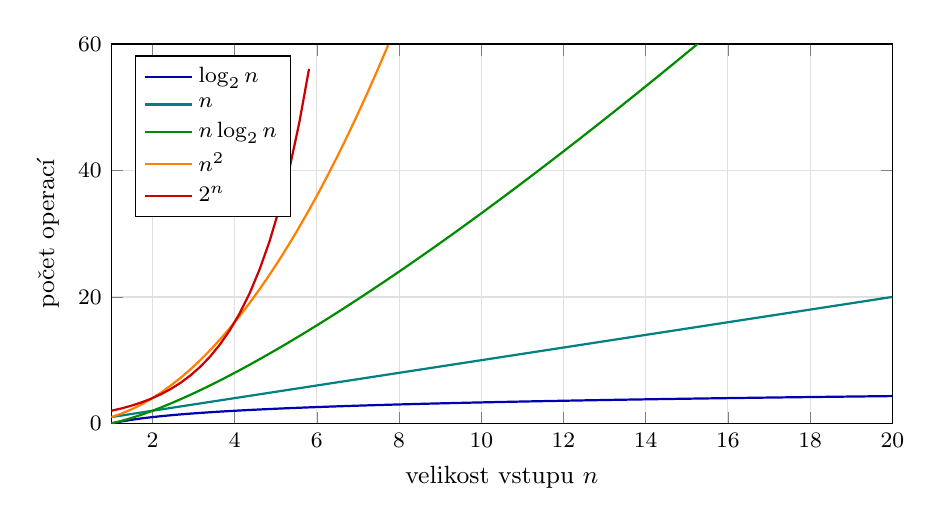
\begin{tikzpicture}
\begin{axis}[
  width=11.5cm,height=6.4cm,
  xlabel={velikost vstupu $n$},ylabel={počet operací},
  domain=1:20,samples=80,
  ymin=0,ymax=60,xmin=1,xmax=20,
  restrict y to domain=0:62,
  legend pos=north west,legend cell align=left,
  grid=both,grid style={black!12},
  tick label style={font=\footnotesize},label style={font=\small},
  legend style={font=\footnotesize},
]
\addplot[blue!70!black,thick]   {ln(x)/ln(2)};      \addlegendentry{$\log_2 n$}
\addplot[teal,thick]            {x};                \addlegendentry{$n$}
\addplot[green!55!black,thick]  {x*ln(x)/ln(2)};    \addlegendentry{$n\log_2 n$}
\addplot[orange,thick]          {x^2};              \addlegendentry{$n^2$}
\addplot[red!80!black,thick]    {2^x};              \addlegendentry{$2^n$}
\end{axis}
\end{tikzpicture}
\end{center}
\obrpopis{růst běžných složitostních funkcí. Pro $n=20$ je $\log_2 n\approx 4{,}3$, $n\log_2 n\approx 86$, $n^2=400$, ale $2^n\approx 10^6$ (vyběhlo z~grafu). Lineární a~linearitmické algoritmy zvládnou obří vstupy; kvadratické jsou na hranici; exponenciální jsou nepoužitelné už pro několik desítek prvků. Zrychlení stroje tisíckrát posune zvládnutelnou velikost u~exponenciálního algoritmu jen o~$\approx\!10$ prvků.}

\begin{priklad}[Určení složitosti dvojitého cyklu]
\textbf{Zadání.} Určete časovou složitost fragmentu: pro $i=1,\dots,n$ a~uvnitř pro $j=i,\dots,n$ proveď konstantní práci.\par
\textbf{Řešení.} Vnitřní tělo se provede $\sum_{i=1}^{n}(n-i+1)=n+(n-1)+\dots+1=\tfrac{n(n+1)}2$ krát. To je $\tfrac12 n^2+\tfrac12 n$; nejrychleji rostoucí člen je $n^2$, konstantu $\tfrac12$ zahodíme, takže složitost je $\boxed{\Theta(n^2)}$. Prostorová složitost je $\Theta(1)$ (jen pár indexů).
\end{priklad}

% ============================================================
\section{Třídy složitosti: P, NP, převoditelnost, NP-úplnost}

Dosud jsme měřili složitost konkrétních algoritmů. Teď se ptáme na složitost \emph{problémů}: existuje pro daný problém efektivní algoritmus vůbec? Hranicí „efektivnosti`` je polynomiální čas. Klíčové je, že u~mnoha praktických úloh efektivní algoritmus \emph{neznáme}, ale ani neumíme dokázat, že neexistuje -- a~tyto úlohy jsou navzájem „stejně těžké`` ve smyslu převoditelnosti. To je obsah teorie NP-úplnosti.

\subsection{Rozhodovací problémy, třídy P a NP}

\begin{definice}[Rozhodovací problém / jazyk]
\emph{Rozhodovací problém} je úloha s~odpovědí ano/ne. Vstup zakódujeme jako řetězec nad abecedou $\{0,1\}$; problém pak ztotožníme s~\emph{jazykem} $L\subseteq\{0,1\}^*$ všech vstupů, na něž je odpověď ano. \emph{Velikostí vstupu} $x$ je délka řetězce $|x|$.
\end{definice}

\begin{definice}[Třída P]
Problém $L$ leží v~třídě \textbf{P}, existuje-li algoritmus $A$ a~polynom $p$ tak, že pro každý vstup $x$ algoritmus $A$ doběhne v~čase nejvýše $p(|x|)$ a~vydá správnou odpověď (tj.\ $A(x)=1\Leftrightarrow x\in L$). Neformálně: \textbf{P} jsou problémy \emph{řešitelné v~polynomiálním čase}.
\end{definice}

\begin{definice}[Třída NP]
Problém $L$ leží v~třídě \textbf{NP}, existuje-li problém $K\in\textbf{P}$ (\emph{verifikátor}) a~polynom $g$ tak, že pro každý vstup $x$ platí
\[
x\in L\ \Longleftrightarrow\ \exists\, y,\ |y|\le g(|x|):\ K(x,y)=1 .
\]
Řetězci $y$ se říká \emph{certifikát} (svědek). Neformálně: \textbf{NP} jsou problémy, u~nichž lze \emph{ověřit} předložené řešení v~polynomiálním čase.
\end{definice}

\begin{intuice}
Rozdíl P vs.\ NP je „najít řešení`` vs.\ „ověřit hotové řešení``. U~SAT (splnitelnost formule) neumíme rychle splňující ohodnocení \emph{najít}, ale dostaneme-li nějaké, snadno ho \emph{ověříme}. Platí $\textbf P\subseteq\textbf{NP}$ (kdo umí řešit, umí i~ověřit -- certifikát ignoruje). Zda je inkluze ostrá, tedy zda $\textbf P\ne\textbf{NP}$, je nejslavnější otevřený problém informatiky.
\end{intuice}

\subsection{Převoditelnost, NP-těžkost a NP-úplnost}

\begin{definice}[Polynomiální převod (redukce)]
Problém $A$ se \emph{polynomiálně převádí} na $B$ (píšeme $A\le B$, případně $A\to B$), existuje-li funkce $f\colon\{0,1\}^*\to\{0,1\}^*$ spočitatelná v~polynomiálním čase taková, že pro každý vstup $x$ platí
\[
x\in A\ \Longleftrightarrow\ f(x)\in B .
\]
\end{definice}

\begin{intuice}
$A\le B$ znamená „$B$ je aspoň tak těžký jako $A$`` -- obtížnost teče po šipce. Kdybychom uměli rychle řešit $B$, uměli bychom rychle řešit i~$A$ (vstup $x$ přeložíme na $f(x)$ a~zeptáme se na~$B$). Převod je \emph{reflexivní} a~\emph{tranzitivní} ($A\le B\le C\Rightarrow A\le C$), tvoří tedy kvaziuspořádání „podle obtížnosti``.
\end{intuice}

\begin{lemma}[Dědičnost snadnosti]
Je-li $A\le B$ a~$B\in\textbf P$, pak $A\in\textbf P$. Důsledkem (obměnou): je-li $A\le B$ a~$A\notin\textbf P$, pak ani $B$ neleží v~\textbf P, tj.\ $B\notin\textbf P$.
\end{lemma}

\begin{definice}[NP-těžkost a NP-úplnost]
Problém $L$ je \textbf{NP-těžký}, pokud se na něj polynomiálně převádí \emph{každý} problém z~\textbf{NP}. Je-li navíc $L\in\textbf{NP}$, je $L$ \textbf{NP-úplný}. NP-úplné problémy jsou tedy „nejtěžší v~NP``.
\end{definice}

\begin{veta}[Cookova--Levinova, bez důkazu]
Problém \textsc{SAT} (splnitelnost výrokové formule v~CNF) je NP-úplný.
\end{veta}

\begin{intuice}
Cookova věta dává „první`` NP-úplný problém. Další NP-úplnost se pak dokazuje \emph{převodem}: chci-li ukázat, že $M\in\textbf{NP}$ je NP-úplný, stačí (1) ověřit $M\in\textbf{NP}$ a~(2) převést nějaký už známý NP-úplný problém $L$ na $M$ ($L\le M$). Z~tranzitivity pak vše z~NP $\le L\le M$.
\end{intuice}

\begin{poznamka}
Mezi klasické NP-úplné problémy patří \textsc{SAT}, \textsc{3-SAT}, nezávislá množina, klika, $k$-barvení grafu ($k\ge3$), Hamiltonovská kružnice, batoh a~součet podmnožiny. Šipky níže ukazují směr typických \emph{převodů} mezi nimi; jeden z~nich, \textsc{3-SAT}~$\to$~nezávislá množina, si vzápětí rozebereme jako příklad:
\end{poznamka}

\begin{center}
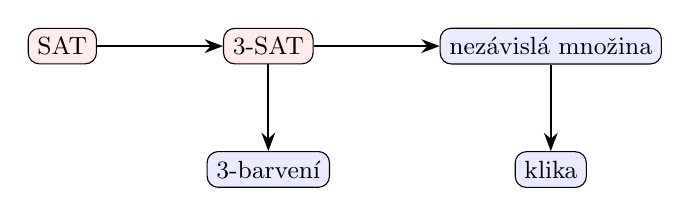
\begin{tikzpicture}[node distance=11mm and 16mm,font=\small]
  \node[draw,rounded corners,fill=red!8] (sat) {SAT};
  \node[draw,rounded corners,fill=red!8,right=of sat] (3sat) {3-SAT};
  \node[draw,rounded corners,fill=blue!8,right=of 3sat] (nz) {nezávislá množina};
  \node[draw,rounded corners,fill=blue!8,below=of nz] (klika) {klika};
  \node[draw,rounded corners,fill=blue!8,below=of 3sat] (barev) {3-barvení};
  \draw[sip] (sat)--(3sat); \draw[sip] (3sat)--(nz);
  \draw[sip] (nz)--(klika); \draw[sip] (3sat)--(barev);
\end{tikzpicture}
\end{center}
\obrpopis{směr převodů $A\to B$ čteme „obtížnost teče po šipce`` ($B$ je aspoň tak těžký jako~$A$). Cookova věta dá NP-úplnost SAT; každá další šipka od~už NP-úplného problému přenáší dál NP-těžkost (tranzitivita převodu) a~spolu s~příslušností cíle do~NP i~NP-úplnost.}

Vztahy tříd za předpokladu $\textbf P\ne\textbf{NP}$ shrnuje obrázek (kdyby $\textbf P=\textbf{NP}$, všechny tři oblasti by splynuly, až na triviální jazyky $\emptyset$ a~$\{0,1\}^*$, které NP-úplné být nemohou):

\begin{center}
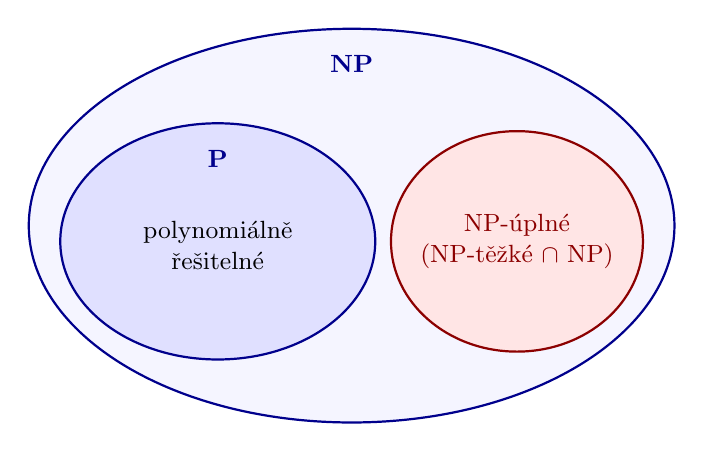
\begin{tikzpicture}[font=\small]
  \draw[fill=blue!4,draw=blue!55!black,thick] (0,0) ellipse (4.1 and 2.5);
  \node[blue!55!black] at (0,2.05) {\textbf{NP}};
  \draw[fill=blue!12,draw=blue!55!black,thick] (-1.7,-0.2) ellipse (2.0 and 1.5);
  \node[blue!55!black] at (-1.7,0.85) {\textbf{P}};
  \draw[fill=red!10,draw=red!55!black,thick] (2.1,-0.2) ellipse (1.6 and 1.4);
  \node[red!55!black,align=center] at (2.1,-0.2) {NP-úplné\\ (NP-těžké $\cap$ NP)};
  \node[align=center] at (-1.7,-0.25) {polynomiálně\\ řešitelné};
\end{tikzpicture}
\end{center}
\obrpopis{$\textbf P\subseteq\textbf{NP}$; NP-úplné problémy leží v~NP, ale (za předpokladu $\textbf P\ne\textbf{NP}$) mimo~P. NP-těžké problémy mohou ležet i~mimo NP (nemusí být ověřitelné v~polynomiálním čase).}

\begin{priklad}[Konkrétní převod: 3-SAT $\to$ nezávislá množina]
\textbf{Zadání.} Ukažte, že problém \textsc{nezávislá množina} (existuje v~grafu $G$ množina aspoň~$k$ vrcholů, z~nichž žádné dva nespojuje hrana?) je NP-úplný. Využijte NP-úplnosti \textsc{3-SAT}.

\smallskip
\textbf{Řešení.}\par
\textbf{(1) Příslušnost do NP.} Certifikátem je samotná $k$-prvková množina vrcholů; ověřit, že žádné dva z~nich nespojuje hrana, zvládneme v~polynomiálním čase. Tedy \textsc{nezávislá množina}~$\in\textbf{NP}$.

\textbf{(2) Převod \textsc{3-SAT}~$\le$~\textsc{nezávislá množina}.} Z~formule $\varphi$ v~3-CNF s~$m$~klauzulemi sestrojíme graf~$G$:
\begin{itemize}
  \item každou klauzuli nahradíme \emph{trojúhelníkem} -- tři vrcholy (po jednom za každý literál klauzule) navzájem pospojované hranami;
  \item mezi vrcholy z~\emph{různých} trojúhelníků přidáme hranu vždy, když jsou jejich literály \emph{kontradiktorické} (tvaru $x_i$ a~$\neg x_i$);
  \item položíme $k=m$.
\end{itemize}
Konstrukce je zjevně polynomiální ($3m$ vrcholů, nejvýše $O(m^2)$ hran).

\begin{center}
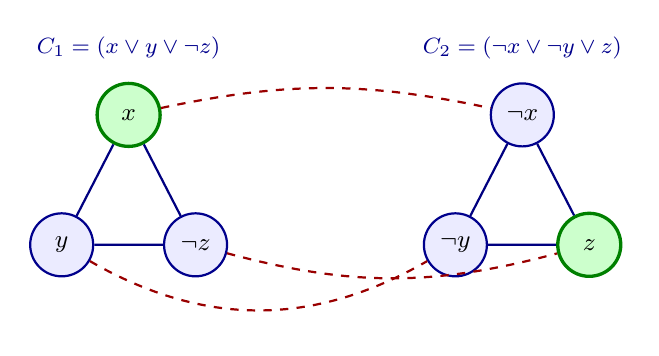
\begin{tikzpicture}[font=\small,
   lit/.style={circle,draw=blue!55!black,fill=blue!8,thick,minimum size=8mm,inner sep=1pt},
   sel/.style={circle,draw=green!50!black,fill=green!20,very thick,minimum size=8mm,inner sep=1pt},
   tri/.style={thick,blue!50!black},
   con/.style={dashed,red!60!black,thick}]
  \node[font=\footnotesize,blue!55!black] at (0,2.35) {$C_1=(x\vee y\vee\neg z)$};
  \node[font=\footnotesize,blue!55!black] at (5,2.35) {$C_2=(\neg x\vee\neg y\vee z)$};
  \node[sel] (x)  at (0,1.5)       {$x$};
  \node[lit] (y)  at (-0.85,-0.15) {$y$};
  \node[lit] (nz) at (0.85,-0.15)  {$\neg z$};
  \draw[tri] (x)--(y) (y)--(nz) (nz)--(x);
  \node[lit] (nx) at (5,1.5)       {$\neg x$};
  \node[lit] (ny) at (4.15,-0.15)  {$\neg y$};
  \node[sel] (z)  at (5.85,-0.15)  {$z$};
  \draw[tri] (nx)--(ny) (ny)--(z) (z)--(nx);
  \draw[con] (x)  to[bend left=12]  (nx);
  \draw[con] (y)  to[bend right=30] (ny);
  \draw[con] (nz) to[bend right=15] (z);
\end{tikzpicture}
\end{center}
\obrpopis{převod formule $\varphi=(x\vee y\vee\neg z)\wedge(\neg x\vee\neg y\vee z)$ na graf. Každá klauzule je trojúhelník (plné hrany); kontradiktorické literály z~různých klauzulí spojuje \emph{čárkovaná} hrana ($x\!-\!\neg x$, $y\!-\!\neg y$, $z\!-\!\neg z$). Hledáme nezávislou množinu velikosti $k=m=2$: zelené vrcholy $\{x,z\}$ jí jsou (z~každého trojúhelníku jeden, navzájem nespojené) a~odpovídají splňujícímu ohodnocení $x=z=1$.}

\textbf{Korektnost:} $\varphi$ je splnitelná $\Leftrightarrow$ $G$ má nezávislou množinu velikosti~$m$.
\begin{itemize}
  \item ($\Rightarrow$) Ze splňujícího ohodnocení vyber v~každé klauzuli jeden \emph{pravdivý} literál a~jeho vrchol. Z~každého trojúhelníku tak bereme právě jeden vrchol (vnitřní hranu neporušíme) a~dva vybrané vrcholy nemohou být kontradiktorické (oba literály jsou pod týmž ohodnocením pravdivé), takže neporušíme ani hranu mezi trojúhelníky. Vznikne nezávislá množina velikosti~$m$.
  \item ($\Leftarrow$) Nezávislá množina velikosti~$m$ musí z~každého trojúhelníku brát \emph{právě jeden} vrchol (trojúhelník je úplný, dva by spojovala hrana). Vybrané literály nastav na \emph{pravdu}; je to bezesporné, neboť dva kontradiktorické literály spojuje hrana, takže oba ve množině být nemohou. Každá klauzule má vybraný, a~tedy pravdivý literál, takže $\varphi$ je splněná.
\end{itemize}
Protože \textsc{3-SAT} je NP-úplný a~\textsc{3-SAT}~$\le$~\textsc{nezávislá množina}, je \textsc{nezávislá množina} NP-těžká; spolu s~bodem~(1) je tedy \textbf{NP-úplná}.
\end{priklad}

\begin{priklad}[SZZ podzim 2025 č.~1: Třídy složitosti (P/NP, redukce, NP-úplnost)]
\szzotazka{podzim 2025}{1}{Třídy složitosti (P/NP, redukce, NP-úplnost)}\par
\textbf{Zadání.}\par
\begin{enumerate}
  \item Definujte třídy složitosti \textbf{P} a~\textbf{NP}.
  \item Definujte převod (redukci) mezi rozhodovacími problémy.
  \item Definujte \textbf{NP}-úplnost rozhodovacího problému.
  \item Rozhodněte, zda následující problém leží v~\textbf{NP}, a~zdůvodněte: je dáno přirozené číslo $x$ v~desítkové soustavě; existují přirozená $a,b$ s~$1<a,b<x$, $x=a\cdot b$ a~desítkové zápisy $a,b$ (bez počátečních nul) jsou stejně dlouhé?
\end{enumerate}

\smallskip
\textbf{Řešení.}\par
\textbf{(1)--(3)} Přesně definice výše: \textbf{P} jsou problémy řešitelné v~polynomiálním čase; \textbf{NP} problémy s~polynomiálně ověřitelným certifikátem; převod $A\le B$ je polynomiální $f$ s~$x\in A\Leftrightarrow f(x)\in B$; $L$ je NP-úplný, je-li NP-těžký (vše z~NP se na něj převádí) a~zároveň $L\in\textbf{NP}$.

\textbf{(4)} \textbf{Velikost vstupu} je počet číslic $x$, tedy $\approx\log_{10}x$ (ne hodnota $x$!). Tvrdíme, že problém \emph{leží v~\textbf{NP}}. Jako \textbf{certifikát} vezmeme jeden z~činitelů $a$. Verifikátor:
\begin{enumerate}
  \item zkontroluje, že $a$ je číslo s~$1<a<x$ a~že $a\mid x$; spočte $b=x/a$ (dělení se zbytkem -- při nenulovém zbytku zamítne),
  \item ověří $1<b<x$ a~že desítkové zápisy $a$ a~$b$ mají stejnou délku.
\end{enumerate}
Délka certifikátu $a$ je nejvýše délka $x$, tedy \emph{lineární} ve velikosti vstupu. Dělení, porovnání a~měření délky zápisů jsou polynomiální v~počtu číslic. Tedy existuje polynomiální verifikátor a~problém je v~\textbf{NP}.

\begin{poznamka}
Pozor na typickou past: kdybychom „velikost`` měřili hodnotou $x$, vyšel by zkoušení dělitelů zdánlivě „polynomiální`` čas $O(x)$. Vůči \emph{počtu číslic} je ale $x$ exponenciální, takže naivní faktorizace polynomiální není. To, že problém je v~NP, plyne z~existence krátkého certifikátu, ne z~rychlého řešení.
\end{poznamka}
\end{priklad}

% ============================================================
\section{Metoda rozděl a panuj (Master theorem)}

\emph{Rozděl a~panuj} je návrhová technika: úlohu rozložíme na několik menších podúloh téhož typu, ty vyřešíme rekurzivně a~jejich výsledky spojíme. Časová složitost se pak řídí \emph{rekurentní rovnicí}, kterou typicky vyřeší Master theorem.

\subsection{Rekurentní rovnice a Master theorem}

Algoritmus, který vstup velikosti $n$ rozdělí na $a$ podproblémů velikosti $n/b$ a~rozdělení i~spojení zvládne v~čase $\Theta(n^c)$, má složitost danou rovnicí
\[
T(n)=a\,T(n/b)+\Theta(n^c),\qquad T(1)=\Theta(1).
\]

\begin{veta}[Master theorem / Kuchařková věta, bez důkazu]
Nechť $a\ge1$, $b>1$, $c\ge0$ jsou konstanty a~$T(n)=a\,T(n/b)+\Theta(n^c)$. Označme $q=a/b^c$. Pak
\[
T(n)=
\begin{cases}
\Theta\!\left(n^{c}\right), & q<1\quad(\text{tj. } c>\log_b a),\\[2pt]
\Theta\!\left(n^{c}\log n\right), & q=1\quad(\text{tj. } c=\log_b a),\\[2pt]
\Theta\!\left(n^{\log_b a}\right), & q>1\quad(\text{tj. } c<\log_b a).
\end{cases}
\]
\end{veta}

\begin{intuice}
Strom rekurze má na každém vrcholu $a$ synů a~$\log_b n$ hladin. Na $i$-té hladině je $a^i$ podproblémů velikosti $n/b^i$, dohromady práce $a^i\cdot\Theta\!\big((n/b^i)^c\big)=\Theta\!\big(n^c\,q^{\,i}\big)$. Sečteme geometrickou řadu s~kvocientem $q=a/b^c$:
\begin{itemize}
  \item $q<1$: dominuje \emph{kořen} (vrchní hladina), práce $\Theta(n^c)$;
  \item $q=1$: všechny hladiny stejně, $\log_b n$ hladin krát $\Theta(n^c)$, tedy $\Theta(n^c\log n)$;
  \item $q>1$: dominují \emph{listy}, kterých je $a^{\log_b n}=n^{\log_b a}$.
\end{itemize}
Rozhoduje tedy souboj mezi „práce na spojení`` ($n^c$) a~„počet listů`` ($n^{\log_b a}$).
\end{intuice}

\begin{center}
\scalebox{1.15}{%
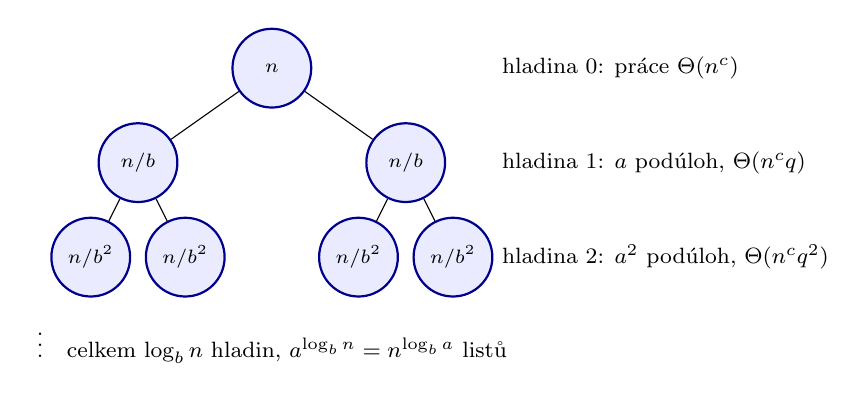
\begin{tikzpicture}[level distance=12mm,font=\footnotesize,
  level 1/.style={sibling distance=34mm},
  level 2/.style={sibling distance=12mm}]
  \tikzset{rn/.style={circle,draw=blue!55!black,fill=blue!8,thick,minimum size=10mm,inner sep=0pt,font=\scriptsize}}
  \node[rn] (r) {$n$}
    child {node[rn] {$n/b$}
      child {node[rn] {$n/b^2$}}
      child {node[rn] {$n/b^2$}}}
    child {node[rn] {$n/b$}
      child {node[rn] {$n/b^2$}}
      child {node[rn] {$n/b^2$}}};
  \node[anchor=west,align=left,font=\footnotesize] at (2.8,0) {hladina $0$: práce $\Theta(n^c)$};
  \node[anchor=west,align=left,font=\footnotesize] at (2.8,-1.2) {hladina $1$: $a$ podúloh, $\Theta(n^c q)$};
  \node[anchor=west,align=left,font=\footnotesize] at (2.8,-2.4) {hladina $2$: $a^2$ podúloh, $\Theta(n^c q^2)$};
  \node[align=center,font=\footnotesize] at (0,-3.45) {$\vdots$\quad celkem $\log_b n$ hladin, $a^{\log_b n}=n^{\log_b a}$ listů};
\end{tikzpicture}}
\end{center}
\obrpopis{strom rekurze pro $T(n)=a\,T(n/b)+\Theta(n^c)$ (zde $a=2$, $b=2$). Součet prací po hladinách je geometrická řada s~kvocientem $q=a/b^c$; který konec řady dominuje, určuje tři případy Master theoremu.}

\subsection{Aplikace I: třídění sléváním (Mergesort) a halda}

\begin{algo}[\textsc{MergeSort} -- třídění sléváním]
\begin{enumerate}
  \item Pokud $n\le1$, vrať vstup. \cmt{triviální případ}
  \item Rozděl posloupnost na dvě poloviny délky $n/2$.
  \item Každou polovinu setřiď rekurzivně voláním \textsc{MergeSort}.
  \item Slij dvě setříděné poloviny do jedné (procedura \textsc{Merge}). \cmt{$\Theta(n)$}
\end{enumerate}
\end{algo}

Procedura \textsc{Merge} porovnává první (nejmenší) prvky obou setříděných posloupností, menší z~nich přesune na výstup a~pokračuje, dokud jednu nevyprázdní; pak zbytek druhé doplní. Každý prvek se přesune právě jednou, takže slévání dvou posloupností o~celkem $n$ prvcích trvá $\Theta(n)$.

Rekurence je $T(n)=2\,T(n/2)+\Theta(n)$, tj.\ $a=2$, $b=2$, $c=1$, $q=2/2^1=1$ -- případ $q=1$, takže
\[
T(n)=\Theta(n\log n).
\]
Prostorová složitost je $\Theta(n)$ (pomocné pole na slévání). Mergesort je \emph{stabilní} (zachová pořadí stejných klíčů, slévá-li se při rovnosti zleva) a~jeho $\Theta(n\log n)$ platí vždy, i~v~nejhorším případě.

Pro slévání více posloupností najednou se hodí \emph{prioritní fronta} realizovaná \emph{haldou}; využijeme ji i~později u~Dijkstry a~Jarníka.

\begin{definice}[Binární halda (prioritní fronta)]
\emph{Binární (minimová) halda} je úplný binární strom uložený v~poli, v~němž platí \emph{haldová podmínka}: klíč každého vrcholu je nejvýše klíče jeho synů (kořen je tedy globální minimum). Podporuje operace \textsc{Insert} (vlož prvek) a~\textsc{ExtractMin} (odeber minimum), obě v~čase $O(\log n)$, a~\textsc{Min} (přečti minimum) v~$O(1)$.
\end{definice}

\begin{priklad}[SZZ léto 2023 č.~1: Třídění sléváním (Mergesort, slévání $k$ posloupností)]
\szzotazka{léto 2023}{1}{Třídění sléváním (Mergesort, slévání $k$ posloupností)}\par
\textbf{Zadání.}
\begin{enumerate}
  \item Formulujte Mergesort v~pseudokódu.
  \item Analyzujte jeho časovou a~prostorovou složitost.
  \item Navrhněte efektivní algoritmus pro slévání $k$ setříděných posloupností o~celkem $n$ prvcích. Upravte Mergesort, aby toto slévání používal. Jak se změní časová složitost (jako funkce $n$ a~$k$)?
\end{enumerate}

\smallskip
\textbf{Řešení.}\par
\textbf{(1)} Pseudokód viz algoritmus \textsc{MergeSort} výše (rozděl na poloviny, setřiď rekurzivně, slij).

\textbf{(2)} Rekurence $T(n)=2T(n/2)+\Theta(n)$ dává $\Theta(n\log n)$ času (Master, případ $q=1$); prostor $\Theta(n)$ na pomocné pole.

\textbf{(3) Slévání $k$ posloupností.} Udržujeme \emph{minimovou haldu} s~$k$ prvky -- po jednom „čele`` z~každé posloupnosti. Opakovaně: vytáhni minimum z~haldy (\textsc{ExtractMin}), zapiš ho na výstup a~na jeho místo vlož další prvek z~téže posloupnosti (\textsc{Insert}). Provedeme celkem $n$ dvojic operací, každá $O(\log k)$ (halda má nejvýše $k$ prvků), takže
\[
\text{slévání } k \text{ posloupností} = \boxed{\Theta(n\log k)}.
\]
\textbf{$k$-cestný Mergesort.} Místo dělení na 2~části dělíme na $k$ částí a~slíváme je výše uvedeným $k$-cestným slíváním. Rekurence je $T(n)=k\,T(n/k)+\Theta(n\log k)$. Strom rekurze má $\log_k n$ hladin, na každé je celková práce slévání $\Theta(n\log k)$, tedy
\[
T(n)=\Theta\!\big(n\log k\cdot \log_k n\big)=\Theta\!\Big(n\log k\cdot\tfrac{\log n}{\log k}\Big)=\boxed{\Theta(n\log n)}.
\]
\textbf{Závěr:} faktor $k$ se vykrátí -- asymptotická složitost zůstává $\Theta(n\log n)$ nezávisle na~$k$. (Volba většího $k$ může v~praxi snížit počet průchodů pamětí, ale řád nezmění.)

\begin{poznamka}
Samotné slévání $k$ posloupností je $\Theta(n\log k)$ a~je to optimální: rozhodnout, ze které z~$k$ posloupností pochází každý další prvek, vyžaduje v~porovnávacím modelu $\Omega(n\log k)$ porovnání (analogie dolního odhadu třídění, sekce~5).
\end{poznamka}
\end{priklad}

\subsection{Aplikace II: násobení dlouhých čísel (Karacuba)}

Násobení dvou $n$-ciferných čísel „školním`` postupem stojí $\Theta(n^2)$. Karacubův algoritmus to zrychlí. Čísla $X,Y$ rozdělíme na horní a~dolní polovinu, $X=A\cdot10^{n/2}+B$, $Y=C\cdot10^{n/2}+D$. Pak
\[
XY = AC\cdot10^{n} + (AD+BC)\cdot10^{n/2} + BD .
\]
Naivně to jsou 4~násobení poloviční délky. Karacubův trik využije identitu
\[
AD+BC = (A+B)(C+D)-AC-BD,
\]
takže stačí jen \emph{tři} násobení: $AC$, $BD$ a~$(A+B)(C+D)$. Rekurence je
\[
T(n)=3\,T(n/2)+\Theta(n),\qquad a=3,\ b=2,\ c=1,\ q=\tfrac{3}{2^1}=\tfrac32>1,
\]
tedy případ $q>1$ a~$T(n)=\Theta\!\big(n^{\log_2 3}\big)\approx\Theta(n^{1{,}585})$ -- výrazně lepší než $n^2$.

\subsection{Aplikace III: medián a Quickselect}

\begin{priklad}[SZZ léto 2024 č.~1: Rozděl a panuj (Master theorem, medián $2n$ čísel)]
\szzotazka{léto 2024}{1}{Algoritmy rozděl a panuj (Master theorem, medián $2n$ čísel)}\par
\textbf{Zadání.}
\begin{enumerate}
  \item Rekurzivní algoritmus $A$ na datech velikosti $n$ ($a,c,x,y\in\mathbb N$, $a>0$, $c>1$): (a)~v~čase $\Theta(n^x)$ vybere $a$ podmnožin velikosti $n/c$; (b)~rekurzivně se zavolá na každou; (c)~v~čase $\Theta(n^y)$ spojí výsledky. Určete (bez důkazu) těsný odhad $T(n)$ v~závislosti na $a,c,x,y$.
  \item Pole $X,Y$ délky $n$ obsahují setříděné posloupnosti $n$ přirozených čísel. Navrhněte algoritmus s~časem $O(\log n)$, který najde medián všech $2n$ čísel, a~metodou z~bodu~1) dokažte složitost.
\end{enumerate}

\smallskip
\textbf{Řešení.}\par
\textbf{(1)} Společná režie kroků (a) a~(c) je $\Theta(n^x+n^y)=\Theta(n^{\max\{x,y\}})$. Položíme $d=\max\{x,y\}$ a~dostaneme rekurenci
\[
T(n)=a\,T(n/c)+\Theta(n^{d}).
\]
(Pozn.\ ke značení: oproti našemu znění Master theoremu zde hraje roli dělitele písmeno $c$, tedy $c\leftrightarrow b$, a~exponent je $d\leftrightarrow$ naše~$c$.) Podle Master theoremu s~poměrem $a/c^{d}$:
\[
T(n)=
\begin{cases}
\Theta(n^{d}), & a/c^{d}<1,\\
\Theta(n^{d}\log n), & a/c^{d}=1,\\
\Theta(n^{\log_c a}), & a/c^{d}>1.
\end{cases}
\]

\textbf{(2) Algoritmus (binární vyhledávání mediánu).} Porovnáme „prostřední`` prvky obou polí, např.\ $x=X[\lfloor(n-1)/2\rfloor]$ a~$y=Y[\lfloor(n-1)/2\rfloor]$ (indexujeme od~0):
\begin{itemize}
  \item Je-li $x<y$: odřízneme prvky \emph{vlevo} od $x$ (je jich $\lfloor(n-1)/2\rfloor$) a~stejný počet prvků \emph{vpravo} od $y$. \textbf{Klíčové:} z~$X$ a~z~$Y$ odebereme \emph{stejný počet} prvků -- odebrané z~$X$ nejsou větší než dolní medián, odebrané z~$Y$ nejsou menší než horní medián (zdůvodnění níže), takže prostřední dvojice zbylých prvků je táž jako u~původní množiny. Voláme rekurzi na zbytek.
  \item Je-li $x>y$: symetricky odřízneme prvky vlevo od $y$ a~stejný počet prvků vpravo od $x$.
  \item Je-li $x=y$: $x$ je (jeden z) medián(ů), konec.
\end{itemize}
Pro $n<3$ dopočítáme medián přímo v~konstantním čase (pro $n=2$ by krok nic neodebral).

\textbf{Proč odřezání nemění medián} (případ $x<y$, $k=\lfloor(n-1)/2\rfloor$; setříděné všech $2n$ čísel označme $z_1\le\dots\le z_{2n}$, mediány jsou $z_n$ a~$z_{n+1}$). Vezměme odebraný prvek $X[i]$, $i<k$. Čísla $\ge X[i]$ jsou aspoň všechna v~$X[i..n{-}1]$ ($n-i\ge n-k+1$ čísel) a~v~$Y[k..n{-}1]$ ($n-k$ čísel, všechna $\ge y>x\ge X[i]$), celkem aspoň $2n-2k+1\ge n+2$. Proto $X[i]\le z_{n-1}\le z_n$. Symetricky pro odebraný $Y[j]$, $j\ge n-k$: čísla $\le Y[j]$ jsou aspoň všechna v~$X[0..k]$ a~$Y[0..j]$, celkem aspoň $(k+1)+(n-k+1)=n+2$, tedy $Y[j]\ge z_{n+2}\ge z_{n+1}$. Odebereme-li $k$ čísel „zdola`` a~$k$ „shora``, prostřední dvojice $z_n,z_{n+1}$ zůstane uprostřed. (Ověřeno i~náhodnými testy včetně opakovaných hodnot.)

\textbf{Složitost metodou z~bodu 1).} V~každém kroku uděláme konstantní práci (přístup k~dvěma prvkům, porovnání, posun indexů) a~zavoláme \emph{jednu} rekurzi na poloviční vstup:
\[
T(n)=1\cdot T(n/2)+\Theta(1),\qquad a=1,\ c=2,\ d=0.
\]
Poměr $a/c^{d}=1/2^0=1$ -- případ $q=1$, tedy $T(n)=\Theta(n^0\log n)=\boxed{\Theta(\log n)}$.
\end{priklad}

\begin{poznamka}
Příbuzná úloha je hledání $k$-tého nejmenšího prvku \emph{nesetříděné} posloupnosti. \textbf{Quickselect} ji řeší jako Quicksort s~jedinou rekurzí: rozdělí prvky podle pivota a~pokračuje jen v~části, kde $k$-tý prvek leží; s~náhodným pivotem má očekávaný čas $\Theta(n)$, v~nejhorším případě $\Theta(n^2)$. \textbf{LinearSelect} (metoda „medián mediánů``) zaručí lineární čas i~v~nejhorším případě: rozdělí prvky do pětic, spočte medián každé, rekurzivně najde medián těchto mediánů a~použije ho jako pivot. Ten zaručí, že obě části mají zhruba nejvýše $\tfrac{7}{10}n$ prvků, takže $T(n)=T(n/5)+T(7n/10)+\Theta(n)=\Theta(n)$ (součet $\tfrac15+\tfrac{7}{10}<1$ dá geometrickou řadu; není to čistý tvar pro Master theorem).
\end{poznamka}

% ============================================================
\section{Binární vyhledávací stromy (BST, AVL)}

Vyhledávací strom je datová struktura pro \emph{dynamickou množinu} klíčů s~operacemi hledání, vkládání a~mazání. Klíče drží uspořádané tak, že operace jdou po jediné cestě od kořene -- jejich cena je tedy úměrná \emph{hloubce} stromu. Celá hra je o~to udržet hloubku malou ($\Theta(\log n)$), což řeší vyvážené stromy (AVL).

\subsection{Binární vyhledávací strom a jeho operace}

\begin{definice}[Binární vyhledávací strom (BST)]
\emph{Binární vyhledávací strom} je binární strom, jehož každý vrchol $v$ nese klíč $k(v)$, a~to tak, že pro každý vrchol platí \emph{uspořádací vlastnost}: všechny klíče v~levém podstromu $v$ jsou $<k(v)$ a~všechny klíče v~pravém podstromu jsou $>k(v)$.
\end{definice}

\begin{intuice}
Vrchol „rozděluje`` zbytek na menší (vlevo) a~větší (vpravo). Hledání klíče $x$ proto jde jednoznačně: porovnej $x$ s~$k(v)$ a~podle výsledku jdi doleva, doprava, nebo jsi našel. Symetrický (in-order) průchod -- nejprve levý podstrom, pak vrchol, pak pravý -- vypíše klíče \emph{vzestupně setříděné}.
\end{intuice}

Operace \textsc{Find}, \textsc{Insert} i~\textsc{Delete} sledují od kořene cestu danou porovnáváním klíčů:
\begin{itemize}
  \item \textsc{Find}$(x)$: v~každém vrcholu jdi doleva/doprava podle porovnání; konec v~nalezeném vrcholu, nebo v~prázdném podstromu (nenalezeno).
  \item \textsc{Insert}$(x)$: jako \textsc{Find}; na místě prázdného podstromu, kde hledání skončilo, vytvoř nový list.
  \item \textsc{Delete}$(x)$: tři případy -- list smaž; vrchol s~jedním synem „přemosti`` synem; vrchol se dvěma syny nahraď jeho \emph{následníkem} (nejlevější vrchol pravého podstromu) a~ten pak smaž (má nejvýše jednoho syna).
\end{itemize}
Všechny tři stojí $\Theta(h)$, kde $h$ je hloubka stromu. V~příznivém (vyváženém) případě je $h=\Theta(\log n)$, v~nejhorším (degenerovaný strom, „liána`` -- vznikne např.\ vkládáním už setříděných klíčů) je $h=\Theta(n)$.

\begin{center}
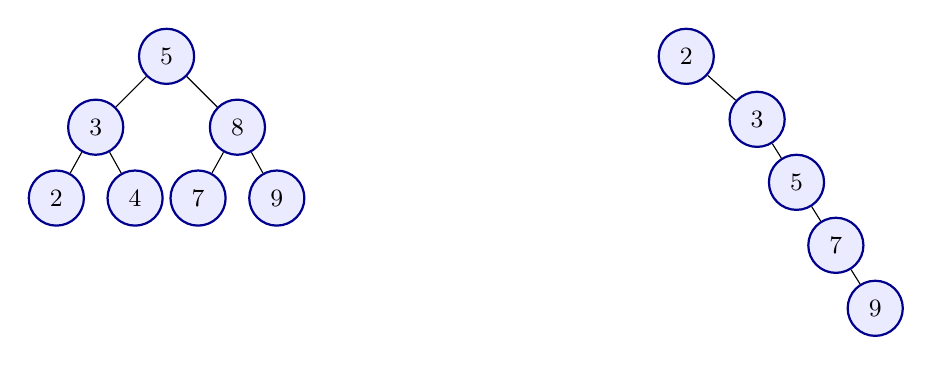
\begin{tikzpicture}[level distance=9mm,font=\small,
  level 1/.style={sibling distance=18mm},
  level 2/.style={sibling distance=10mm}]
\begin{scope}
  \node[bst] {5}
    child {node[bst] {3} child {node[bst] {2}} child {node[bst] {4}}}
    child {node[bst] {8} child {node[bst] {7}} child {node[bst] {9}}};
\end{scope}
\begin{scope}[xshift=6.6cm,level distance=8mm]
  \node[bst] (a) {2}
    child[missing]
    child {node[bst] (b) {3}
      child[missing]
      child {node[bst] (c) {5}
        child[missing]
        child {node[bst] (d) {7}
          child[missing]
          child {node[bst] (e) {9}}}}};
\end{scope}
\end{tikzpicture}
\end{center}
\obrpopis{vlevo \emph{vyvážený} BST na 7~vrcholech, hloubka $2=\lfloor\log_2 7\rfloor$, operace $\Theta(\log n)$. Vpravo \emph{degenerovaný} BST („liána``) ze stejných klíčů vložených v~setříděném pořadí $2,3,5,7,9$: hloubka $n-1$, operace $\Theta(n)$. Oba splňují uspořádací vlastnost (levý $<$ vrchol $<$ pravý); liší se jen tvarem -- proto chceme tvar řídit (AVL).}

\subsection{AVL stromy}

\begin{definice}[AVL strom]
\emph{AVL strom} je binární vyhledávací strom, který je \emph{hloubkově vyvážený}: pro každý vrchol $v$ se hloubky jeho levého a~pravého podstromu liší nejvýše o~1, tj.
\[
\bigl|\,h(\ell(v))-h(r(v))\,\bigr|\le 1 .
\]
V~každém vrcholu si pamatujeme \emph{znaménko} (balanci) $\delta(v)=h(r(v))-h(\ell(v))\in\{-1,0,+1\}$.
\end{definice}

\begin{veta}[Hloubka AVL stromu]
AVL strom o~$n$ vrcholech má hloubku $\Theta(\log n)$.
\end{veta}

\begin{intuice}
Dolní mez $h\ge\log_2(n+1)-1$ platí pro každý binární strom (strom hloubky $h$ má nejvýše $2^{h+1}-1$ vrcholů). Podstatná je \emph{horní} mez hloubky, tedy \emph{dolní mez na počet vrcholů}: označme $A_h$ nejmenší možný počet vrcholů AVL stromu hloubky~$h$. Kořen má dva podstromy, jeden hloubky $h-1$ a~(aby byl strom co nejřidší) druhý hloubky $h-2$, takže
\[
A_h=A_{h-1}+A_{h-2}+1,\qquad A_0=1,\ A_1=2.
\]
To je posloupnost Fibonacciho typu, $A_h=F_{h+3}-1$, a~roste exponenciálně: $A_h\ge \varphi^{\,h}$ pro $\varphi=\tfrac{1+\sqrt5}{2}$. Tedy $n\ge A_h\ge\varphi^h$, odkud $h\le\log_\varphi n=\Theta(\log n)$. AVL strom je proto vždy „skoro vyvážený`` a~všechny operace stojí $\Theta(\log n)$.
\end{intuice}

Vyváženost se po vložení nebo smazání obnovuje \emph{rotacemi} -- lokálními přepojeními, která zachovají uspořádací vlastnost a~zmenší hloubku rozhozeného místa. Stačí $O(1)$ rotací na jedné hladině, propagace nahoru je $O(\log n)$.

\begin{center}
\scalebox{1.1}{%
\begin{tikzpicture}[font=\small,
   nd/.style={circle,draw=blue!55!black,fill=blue!8,thick,minimum size=7mm,inner sep=0pt},
   tri/.style={isosceles triangle,draw=blue!45!black,fill=blue!4,shape border rotate=90,
               minimum width=8mm,minimum height=6.5mm,inner sep=0pt,font=\footnotesize,anchor=north}]
  % --- pred rotaci (vlevo): rozhozeni vlevo-vlevo, delta(y) = -2 ---
  \node[nd]  (y1) at (0,2)       {$y$};
  \node[nd]  (x1) at (-1,1)      {$x$};
  \node[tri] (C1) at (1,1.1)     {$C$};
  \node[tri] (A1) at (-1.6,0.15) {$A$};
  \node[tri] (B1) at (-0.4,0.15) {$B$};
  \draw[thick] (y1)--(x1) (y1)--(C1) (x1)--(A1) (x1)--(B1);
  \node[font=\footnotesize] at (-0.3,-1.15) {před: $\delta(y)=-2$};
  % --- sipka ---
  \node at (2.7,1) {$\xrightarrow{\ \text{rotace}\ }$};
  % --- po rotaci (vpravo): vyvazeno ---
  \begin{scope}[xshift=5.2cm]
   \node[nd]  (x2) at (0,2)      {$x$};
   \node[tri] (A2) at (-1,1.1)   {$A$};
   \node[nd]  (y2) at (1,1)      {$y$};
   \node[tri] (B2) at (0.4,0.15) {$B$};
   \node[tri] (C2) at (1.6,0.15) {$C$};
   \draw[thick] (x2)--(A2) (x2)--(y2) (y2)--(B2) (y2)--(C2);
   \node[font=\footnotesize] at (0.3,-1.15) {po: $\delta=0$, hloubka $-1$};
  \end{scope}
\end{tikzpicture}}
\end{center}
\obrpopis{\emph{jednoduchá rotace} hrany $xy$ vyrovná stav $\delta(y)=-2$ s~„rozhozením vlevo-vlevo`` (údaje „po`` platí pro typickou situaci po vložení, kdy $h(A)=h(B)+1$). Podstrom $B$ změní rodiče z~$x$ na~$y$; pořadí klíčů $A<x<B<y<C$ zůstává. (Pro „cik-cak`` rozhození vlevo-vpravo se použije \emph{dvojitá} rotace = dvě jednoduché za sebou.)}

\begin{priklad}[SZZ jaro 2023 č.~1: Třídění pomocí BST a AVL]
\szzotazka{jaro 2023}{1}{Třídění (BST/AVL, složitost)}\par
\textbf{Zadání.}
\begin{enumerate}
  \item Popište, jak pomocí BST setřídit (vzestupně) posloupnost $x_1,\dots,x_n$ navzájem různých prvků.
  \item Co se změní, mohou-li se prvky opakovat?
  \item Co z~toho plyne pro minimální možnou složitost operací s~vyhledávacím stromem, lze-li klíče jen porovnávat?
  \item Jakou složitost má algoritmus z~bodu~1 s~AVL stromem, jsou-li prvky řetězce délky~$L$?
\end{enumerate}

\smallskip
\textbf{Řešení.}\par
\textbf{(1)} Postupně vlož $x_1,\dots,x_n$ do (zprvu prázdného) BST, pak proveď in-order průchod -- ten vypíše klíče vzestupně. Vkládání jednoho prvku stojí $\Theta(h)$; při použití \emph{vyváženého} stromu je $h=\Theta(\log n)$, takže $n$ vložení trvá $\Theta(n\log n)$ a~in-order průchod $\Theta(n)$. Celkem $\boxed{\Theta(n\log n)}$. (S~nevyváženým BST hrozí degenerace na liánu a~čas až $\Theta(n^2)$, např.\ pro už setříděný vstup.)

\textbf{(2)} Při opakování klíčů uspořádací vlastnost „$<$ vlevo, $>$ vpravo`` nestačí. Buď ve vrcholu držíme \emph{počet výskytů} klíče (in-order pak vypíše klíč tolikrát), nebo povolíme rovnost na jedné straně ($\le$), případně klíče zjednoznačníme dvojicí $(x_i,i)$ porovnávanou lexikograficky (to navíc dá stabilní třídění). Setřídění zůstane $\Theta(n\log n)$; výstup už není množina, ale multimnožina.

\textbf{(3)} Třídění stromem je $n$-krát \textsc{Insert} a~jeden in-order výpis; výpis stojí $O(n)$ a~žádná porovnání nepotřebuje. Kdyby nějaký vyhledávací strom (v~porovnávacím modelu) zvládl $n$ vložení v~čase $o(n\log n)$, uměli bychom porovnáváním třídit v~čase $o(n\log n)$. To zakazuje dolní odhad porovnávacího třídění (sekce~5): $\Omega(n\log n)$ porovnání v~nejhorším případě. Proto \textsc{Insert} nemůže mít (ani amortizovaně) složitost $o(\log n)$; potřebuje $\Omega(\log n)$ porovnání. Logaritmická cena operací AVL stromu je tedy v~tomto smyslu \emph{optimální}.

\textbf{(4)} U~řetězců délky $L$ není jedno porovnání konstantní -- porovnání dvou řetězců stojí až $\Theta(L)$ (znak po znaku). Vkládání jednoho řetězce do AVL stromu projde $\Theta(\log n)$ vrcholů, v~každém jedno porovnání řetězců za $O(L)$, tedy $O(L\log n)$ na prvek a~$O(nL\log n)$ za $n$ vložení. In-order výpis vypíše $n$ řetězců o~celkové délce $\le nL$ za $O(nL)$. Celková složitost je
\[
\boxed{O(nL\log n)} .
\]
\end{priklad}

\begin{poznamka}
Plně rozkreslené stromy (vyvážený vs.\ liána, in-order pořadí, průběh rotace při vkládání) jsou v~\texttt{priklady/} u~této otázky.
\end{poznamka}

\begin{priklad}[SZZ léto 2022 č.~1: Binární vyhledávací stromy]
\szzotazka{léto 2022}{1}{Binární vyhledávací stromy}\par
\textbf{Zadání.} (1)~Definujte binární vyhledávací strom (BVS). (2)~Pseudokódem implementujte \emph{vložení} prvku (bez vyvažování) a~rozeberte časovou složitost v~nejlepším a~nejhorším případě. (3)~Pseudokódem implementujte nalezení \emph{následníka} (pro klíč $x$ vrchol s~nejmenším klíčem $>x$) a~rozeberte složitost v~nejlepším a~nejhorším případě.

\smallskip
\textbf{Řešení.}\par
\textbf{(1)} BVS je binární strom, jehož každý vrchol nese klíč a~splňuje \emph{uspořádací vlastnost}: všechny klíče v~levém podstromu jsou $<$ klíč vrcholu a~všechny v~pravém podstromu jsou $>$ klíč vrcholu (viz definice výše).

\textbf{(2) Vložení.} Sestup od kořene doleva/doprava podle porovnání; nový prvek vlož jako list tam, kde sestup narazí na prázdný podstrom.
\begin{lstlisting}
Insert(strom T, klic k):
  if T.koren == null:
    T.koren = new Uzel(k); return
  v = T.koren
  loop:
    if k == v.klic: return      // klic uz ve strome je
    if k < v.klic:
      if v.levy == null: v.levy = new Uzel(k); return
      else: v = v.levy
    else:                       // k > v.klic
      if v.pravy == null: v.pravy = new Uzel(k); return
      else: v = v.pravy
\end{lstlisting}
Vložení projde jedinou cestu od kořene nejvýše k~listu, tj.\ $O(h)$, a~v~nejhorším případě (nový list pod nejhlubším listem) $\Theta(h)$. Nejhorší případ: degenerovaný strom (liána, např.\ vzniklý vkládáním setříděné posloupnosti) má $h=n-1$, tedy $\boxed{\Theta(n)}$. Nejlepší případ: sestup skončí hned pod kořenem, tj.\ $\boxed{\Theta(1)}$ (např.\ do liány $1,2,\dots,n$ vkládáme $0$). Chceme-li nejlepší \emph{tvar stromu} při nejhorší volbě klíče, je to vyvážený strom s~$h=\Theta(\log n)$, tedy $\Theta(\log n)$.

\textbf{(3) Následník.} Má-li $x$ pravý podstrom, následník je jeho nejlevější vrchol; jinak stoupej nahoru, dokud nejsi levým synem -- ten rodič je následník (jinak byl $x$ maximem).
\begin{lstlisting}
Successor(uzel x):
  if x.pravy != null:                 // nejmensi v pravem podstromu
    v = x.pravy
    while v.levy != null: v = v.levy
    return v
  v = x; r = x.rodic                  // nahoru, dokud nejsem levy syn
  while r != null and v == r.pravy:
    v = r; r = r.rodic
  return r
\end{lstlisting}
Obě větve projdou jednu cestu, takže $O(h)$. Nejhorší případ $\Theta(n)$: ve stromu vzniklém vkládáním $1,n,n-1,\dots,2$ je následník kořene~$1$ klíč~$2$ na dně levé větve pod~$n$, cesta má $n-1$ hran. Nejlepší případ $\Theta(1)$ (pravý syn $x$ je list, nebo $x$ je levý syn bez pravého podstromu). Ve vyváženém stromu je i~nejhorší případ jen $\Theta(\log n)$.
\end{priklad}

% ============================================================
\section{Třídění: primitivní algoritmy, Quicksort, dolní odhad}

Třídění je nejčastější podúloha vůbec. Projdeme jednoduché kvadratické algoritmy, praktický Quicksort a~dokážeme, že porovnávací třídění nejde rychleji než $\Theta(n\log n)$.

\subsection{Primitivní třídicí algoritmy}

Dvě pomocná pojmenování: \emph{inverze} je dvojice indexů $i<j$ s~$a_i>a_j$ (prvky ve špatném vzájemném pořadí); třídicí algoritmus je \emph{stabilní}, zachovává-li vzájemné pořadí prvků se \emph{stejným} klíčem.

\begin{itemize}
  \item \textbf{Selectsort (výběrem):} opakovaně najdi minimum nesetříděné části a~dej ho na konec setříděné. Vždy $\Theta(n^2)$ porovnání; prostor $\Theta(1)$; nestabilní.
  \item \textbf{Insertsort (vkládáním):} ber prvky po jednom a~vsouvej je na správné místo do už setříděné přední části (posouváním). Nejhorší/průměrný $\Theta(n^2)$, \emph{nejlepší $\Theta(n)$} (téměř setříděný vstup); prostor $\Theta(1)$; stabilní.
  \item \textbf{Bubblesort (bublinkové):} opakovaně procházej pole a~prohazuj sousedy ve špatném pořadí; větší prvky „bublají`` dozadu. Nejhorší/průměrný $\Theta(n^2)$, nejlepší $\Theta(n)$ (s~detekcí, že proběhl průchod beze změny); prostor $\Theta(1)$; stabilní.
\end{itemize}

\begin{intuice}
Insertsort a~Bubblesort jsou v~nejhorším případě $\Theta(n^2)$, protože prohazují jen \emph{sousední} prvky, a~každé takové prohození opraví právě jednu inverzi; inverzí přitom může být až $\binom n2=\Theta(n^2)$ (úplně obrácená posloupnost). Selectsort prohazuje i~vzdálené prvky, je ale $\Theta(n^2)$ kvůli počtu porovnání při hledání minim. Pro malá $n$ nebo skoro setříděná data jsou ale rychlé a~jednoduché; Insertsort je proto často „dokončovací`` fáze rychlejších algoritmů.
\end{intuice}

\subsection{Quicksort}

\begin{algo}[\textsc{QuickSort}]
\begin{enumerate}
  \item Pokud $n\le1$, vrať vstup.
  \item Zvol \emph{pivot} $p$ (některý prvek).
  \item Rozděl prvky na $L$ (menší než $p$), $S$ (rovné $p$), $P$ (větší než $p$). \cmt{$\Theta(n)$}
  \item Rekurzivně setřiď $L$ a~$P$.
  \item Vrať zřetězení $L,\,S,\,P$.
\end{enumerate}
\end{algo}

Quicksort je rovněž typu rozděl a~panuj, ale dělení je \emph{datově závislé} (podle pivota). Při „šťastné`` volbě pivota (medián) je rekurence $T(n)=2T(n/2)+\Theta(n)=\Theta(n\log n)$. Při „nešťastné`` volbě (pivot je vždy minimum/maximum -- nastane např.\ na setříděném vstupu s~pivotem na kraji) se odděluje po jednom prvku a~rekurence degeneruje na $T(n)=T(n-1)+\Theta(n)=\Theta(n^2)$.
\[
\text{nejhorší případ } \Theta(n^2),\qquad \text{průměrný případ } \Theta(n\log n).
\]
Náhodná volba pivota dává očekávaný čas $\Theta(n\log n)$ a~v~praxi je Quicksort díky malým konstantám a~třídění „na místě`` zpravidla nejrychlejší. (Verze v~boxu výše pro názornost tvoří nová pole $L,S,P$; praktická implementace dělí pole na místě a~potřebuje jen zásobník rekurze, který má velikost $O(\log n)$, zanořuje-li se rekurze nejdřív do menší části a~větší zpracuje cyklem.) Není stabilní.

\begin{priklad}[Simulace Quicksortu]
\textbf{Zadání.} Odsimulujte Quicksort na poli $[5,3,8,4,2,7,1]$, pivot vždy první prvek.\par
\textbf{Řešení.} V~každém kroku pivot $p$ rozdělí pole na $L<p$, $S=p$, $P>p$; rekurze na $L$ a~$P$.
\begin{itemize}
  \item $[5,3,8,4,2,7,1]$, $p=5$: $L=[3,4,2,1]$, $S=[5]$, $P=[8,7]$.
  \item $[3,4,2,1]$, $p=3$: $L=[2,1]$, $S=[3]$, $P=[4]$; \quad $[2,1]$, $p=2$: $L=[1]$, $S=[2]$, $P=[\,]$.
  \item $[8,7]$, $p=8$: $L=[7]$, $S=[8]$, $P=[\,]$.
\end{itemize}
Zřetězením setříděných částí zdola nahoru dostaneme $\boxed{[1,2,3,4,5,7,8]}$. (Vstup nebyl setříděný, takže pivoty dělily rozumně; na již setříděném vstupu by pivot „první prvek`` byl pokaždé minimum a~strom rekurze by degeneroval na hloubku $n$, tedy $\Theta(n^2)$.)
\end{priklad}

\subsection{Dolní odhad složitosti porovnávacího třídění}

\begin{veta}[Dolní odhad porovnávacího třídění]
Každý deterministický třídicí algoritmus, který o~prvcích zjišťuje informaci \emph{pouze jejich vzájemným porovnáváním}, provede v~nejhorším případě $\Omega(n\log n)$ porovnání.
\end{veta}

\begin{intuice}
Algoritmus „nevidí`` hodnoty, jen výsledky porovnání. Jeho běh popíšeme \emph{rozhodovacím stromem}: vnitřní vrchol = jedno porovnání $a_i$ vs.\ $a_j$ se třemi výsledky ($<,=,>$), list = konečná odpověď (konkrétní setříděné pořadí). Délka cesty k~listu = počet porovnání na daném vstupu, hloubka stromu = nejhorší případ.
\end{intuice}

\begin{proof}[Důkaz (přes rozhodovací strom).]
\begin{enumerate}[label=(\arabic*)]
  \item Uvažme $n$ navzájem různých prvků. Různá vstupní pořadí (permutace) vyžadují různé posloupnosti přesunů, tedy musí skončit v~\emph{různých listech}. Permutací je $n!$, takže rozhodovací strom má aspoň $n!$ listů.
  \item Strom je \emph{ternární} (každý vnitřní vrchol má nejvýše 3~syny dle výsledku porovnání), takže strom hloubky $h$ má nejvýše $3^h$ listů. Z~$3^h\ge n!$ plyne $h\ge\log_3(n!)$.
  \item Odhadneme $\log_3(n!)$ zdola. Z~$n!\ge\left(\tfrac n2\right)^{n/2}$ (aspoň polovina činitelů je $\ge\tfrac n2$) dostaneme
  \[
  h\ge\log_3(n!)\ \ge\ \tfrac n2\log_3\tfrac n2\ =\ \Omega(n\log n).
  \]
\end{enumerate}
Tedy v~nejhorším případě je potřeba $\Omega(n\log n)$ porovnání.
\end{proof}

\begin{center}
\scalebox{1.0}{%
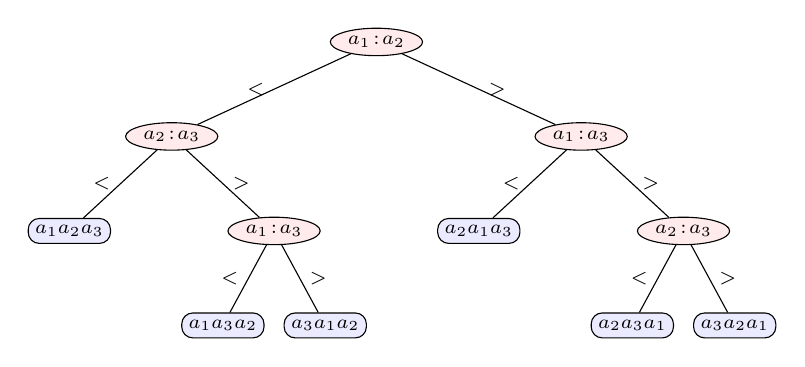
\begin{tikzpicture}[level distance=12mm,font=\scriptsize,
  level 1/.style={sibling distance=52mm},
  level 2/.style={sibling distance=26mm},
  level 3/.style={sibling distance=13mm},
  cmp/.style={draw,ellipse,fill=red!8,inner sep=1.5pt},
  leaf/.style={draw,rounded corners,fill=blue!8,inner sep=2.5pt},
  el/.style={font=\scriptsize}]
  \node[cmp] {$a_1\!:\!a_2$}
    child {node[cmp] {$a_2\!:\!a_3$}
      child {node[leaf] {$a_1a_2a_3$} edge from parent node[el,left]{$<$}}
      child {node[cmp] {$a_1\!:\!a_3$}
        child {node[leaf] {$a_1a_3a_2$} edge from parent node[el,left]{$<$}}
        child {node[leaf] {$a_3a_1a_2$} edge from parent node[el,right]{$>$}}
        edge from parent node[el,right]{$>$}}
      edge from parent node[el,left]{$<$}}
    child {node[cmp] {$a_1\!:\!a_3$}
      child {node[leaf] {$a_2a_1a_3$} edge from parent node[el,left]{$<$}}
      child {node[cmp] {$a_2\!:\!a_3$}
        child {node[leaf] {$a_2a_3a_1$} edge from parent node[el,left]{$<$}}
        child {node[leaf] {$a_3a_2a_1$} edge from parent node[el,right]{$>$}}
        edge from parent node[el,right]{$>$}}
      edge from parent node[el,right]{$>$}};
\end{tikzpicture}}
\end{center}
\obrpopis{úplný rozhodovací strom pro třídění $n=3$ navzájem různých prvků (výsledek „$=$`` proto nenastává). Vnitřní vrcholy jsou porovnání $a_i\!:\!a_j$, hrany jejich výsledky $<,>$ a~listy všech $n!=6$ setříděných pořadí (každé právě jednou). Nejdelší cesta má 3~porovnání, tj.\ hloubka stromu je~3. Obecně $\ge n!$ listů vynutí hloubku $\ge\log_3(n!)=\Omega(n\log n)$; \emph{Mergesort této meze dosahuje}, je tedy asymptoticky optimální.}

\begin{poznamka}
Dolní odhad platí jen v~\emph{porovnávacím} modelu. Třídění, které o~klíčích ví víc (např.\ že jsou to malá celá čísla), může být rychlejší -- přihrádkové (counting/radix) třídění běží až v~$\Theta(n)$, protože klíče neporovnává, ale přímo indexuje.
\end{poznamka}

% ============================================================
\section{Grafové algoritmy}

Graf $G=(V,E)$ modeluje vztahy mezi objekty. Reprezentujeme ho buď \emph{maticí sousednosti} ($n\times n$, test hrany $O(1)$, ale prostor $\Theta(n^2)$ a~výpis sousedů $\Theta(n)$), nebo \emph{seznamy sousedů} (prostor $\Theta(n+m)$, výpis sousedů úměrný jejich počtu) -- pro řídké grafy volíme seznamy. Skoro všechny základní algoritmy pak běží v~čase $O(n+m)$.

\subsection{Prohledávání do šířky (BFS) a do hloubky (DFS)}

\begin{algo}[\textsc{BFS} -- prohledávání do šířky z~$v_0$]
\begin{enumerate}
  \item Všem vrcholům nastav stav \emph{nenalezený}; stav$(v_0)\leftarrow$ \emph{otevřený}, $D(v_0)\leftarrow0$, vlož $v_0$ do fronty $Q$.
  \item Dokud $Q\ne\emptyset$: vyber $v$ ze začátku $Q$.
  \item Pro každého souseda $w$ vrcholu $v$, je-li \emph{nenalezený}: stav$(w)\leftarrow$ \emph{otevřený}, $D(w)\leftarrow D(v)+1$, $P(w)\leftarrow v$, přidej $w$ na konec $Q$. Pak stav$(v)\leftarrow$ \emph{uzavřený}. \cmt{každý vrchol jde do fronty nejvýše jednou}
\end{enumerate}
\end{algo}

BFS prochází vrcholy po \emph{vrstvách} podle vzdálenosti od $v_0$ (počet hran) a~používá \emph{frontu} (FIFO). Vydá vzdálenosti $D(v)$ (nejkratší v~počtu hran) a~strom nejkratších cest přes ukazatele $P$.

\textbf{DFS} (prohledávání do hloubky) naopak používá \emph{zásobník} / rekurzi: z~vrcholu se zanoří co nejhlouběji, než se vrátí. Každému vrcholu přiřadí čas \emph{otevření} $\mathrm{in}(v)$ a~\emph{uzavření} $\mathrm{out}(v)$; tyto časy se chovají jako \emph{závorkování} (podstromy se do sebe vnořují, nekříží).

\begin{algo}[\textsc{DFS} -- prohledávání do hloubky, rekurzivně z~$v_0$]
Globální čítač $T\leftarrow0$; všem vrcholům nastav stav \emph{nenalezený}. Zavolej \textsc{DFS-navštiv}$(v_0)$.
\smallskip

\noindent\textsc{DFS-navštiv}$(v)$:
\begin{enumerate}
  \item $T\leftarrow T+1$; $\mathrm{in}(v)\leftarrow T$; stav$(v)\leftarrow$ \emph{otevřený}.
  \item Pro každého souseda $w$ vrcholu $v$: je-li $w$ \emph{nenalezený}, $P(w)\leftarrow v$ a~zavolej \textsc{DFS-navštiv}$(w)$.
  \item $T\leftarrow T+1$; $\mathrm{out}(v)\leftarrow T$; stav$(v)\leftarrow$ \emph{uzavřený}.
\end{enumerate}
\end{algo}

Obě prohledávání běží v~čase $\Theta(n+m)$ (každý vrchol i~hrana se zpracují konstanta-krát). Časy $\mathrm{in}/\mathrm{out}$ z~DFS využijeme vzápětí u~topologického třídění.

\begin{center}
\scalebox{1.1}{%
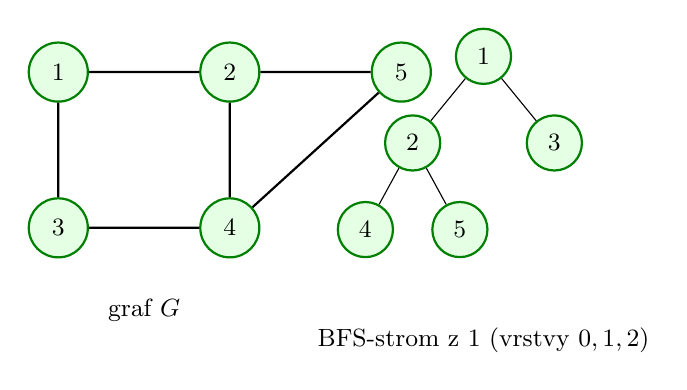
\begin{tikzpicture}[font=\small]
  % graf G
  \node[vrchG] (a) {1};
  \node[vrchG] (b) [right=14mm of a] {2};
  \node[vrchG] (c) [below=12mm of a] {3};
  \node[vrchG] (d) [right=14mm of c] {4};
  \node[vrchG] (e) [right=14mm of b] {5};
  \draw[hrana] (a)--(b) (a)--(c) (b)--(d) (c)--(d) (b)--(e) (d)--(e);
  \node[font=\small] at ($(c)!0.5!(d)+(0,-1.05)$) {graf $G$};
  % BFS strom z 1
  \begin{scope}[xshift=5.4cm,yshift=2mm,level distance=11mm,
     level 1/.style={sibling distance=18mm},
     level 2/.style={sibling distance=12mm},
     every node/.style={vrchG,minimum size=7mm}]
   \node (t1) {1}
     child {node {2}
       child {node {4}}
       child {node {5}}}
     child {node {3}};
  \end{scope}
  \node[font=\small] at (5.4,-3.4) {BFS-strom z~1 (vrstvy $0,1,2$)};
\end{tikzpicture}}
\end{center}
\obrpopis{BFS z~vrcholu~1 dá vrstvy $V_0=\{1\}$, $V_1=\{2,3\}$, $V_2=\{4,5\}$, tj.\ $D=(0,1,1,2,2)$. Stromové hrany (přes které se vrcholy poprvé objevily) tvoří strom nejkratších cest. DFS z~1 by naopak nejdřív sestoupilo $1\!\to\!2\!\to\!4\!\to\!\dots$ a~vracelo se -- pořadí návštěv i~tvar stromu se liší.}

\subsection{Topologické třídění orientovaných grafů}

\begin{definice}[DAG a topologické uspořádání]
\emph{Orientovaný acyklický graf} (DAG) je orientovaný graf bez orientovaného cyklu. \emph{Topologické uspořádání} je lineární uspořádání $\prec$ vrcholů takové, že pro každou hranu $uv$ platí $u\prec v$ (každá hrana míří „dopředu``).
\end{definice}

\begin{veta}[Existence topologického uspořádání]
Orientovaný graf má topologické uspořádání právě tehdy, když je to DAG. Uspořádání lze najít v~čase $\Theta(n+m)$.
\end{veta}

\begin{intuice}
Cyklus zjevně topologicky uspořádat nelze (po šipkách bychom se vrátili). V~DAGu naopak vždy existuje vrchol bez vstupních hran (zdroj); ten dáme první a~odebereme -- a~indukcí pokračujeme. Algoritmicky elegantnější: spusť DFS; pořadí \emph{klesajících} časů uzavření $\mathrm{out}(v)$ je topologické. (Pro každou hranu $uv$ v~DAGu totiž $\mathrm{out}(u)>\mathrm{out}(v)$, protože zpětné hrany, které by to porušily, by tvořily cyklus.)
\end{intuice}

\begin{center}
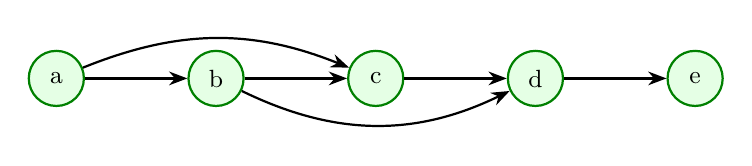
\begin{tikzpicture}[font=\small,>=Stealth,every node/.style={vrchG,minimum size=7mm},node distance=13mm]
  \node (a) {a}; \node (b) [right=of a] {b}; \node (c) [right=of b] {c};
  \node (d) [right=of c] {d}; \node (e) [right=of d] {e};
  \draw[sip] (a)--(b); \draw[sip] (a) to[bend left=22] (c);
  \draw[sip] (b)--(c); \draw[sip] (b) to[bend right=26] (d);
  \draw[sip] (c)--(d); \draw[sip] (d)--(e);
\end{tikzpicture}
\end{center}
\obrpopis{DAG srovnaný do řady $a\prec b\prec c\prec d\prec e$ -- všechny hrany míří zleva doprava, což je přesně topologické uspořádání. Takové uspořádání umožní počítat na DAGu „po proudu`` (např.\ nejdelší cestu, počet cest) v~lineárním čase.}

\subsection{Nejkratší cesty v ohodnocených grafech}

Mějme graf s~délkami hran $\ell(e)$. \emph{Vzdálenost} $d(u,v)$ je nejmenší délka $uv$-sledu. Je dobře definovaná, pokud v~grafu nejsou \emph{záporné cykly} (obcházením by šlo sled libovolně zkracovat); pak se minimum nabývá na cestě. Oba následující algoritmy stojí na \emph{relaxaci} hrany: je-li $h(w)>h(v)+\ell(vw)$, zlepši $h(w)\leftarrow h(v)+\ell(vw)$.

\begin{veta}[Dijkstrův algoritmus]
Pro graf s~\emph{nezápornými} délkami hran najde Dijkstrův algoritmus vzdálenosti z~$v_0$ do všech vrcholů. S~binární haldou běží v~čase $O\big((n+m)\log n\big)$.
\end{veta}

\begin{intuice}
Dijkstra uzavírá vrcholy v~pořadí rostoucí vzdálenosti: vždy vytáhne dosud neuzavřený vrchol s~nejmenším $h$ (proto halda) a~zrelaxuje jeho hrany. Klíčový invariant: jakmile vrchol uzavřeme, jeho $h$ už je správná vzdálenost a~vrchol se znovu neotevře -- to platí právě proto, že hrany jsou nezáporné (objížďka přes pozdější, vzdálenější vrchol nemůže být kratší). Proto se každý vrchol uzavře jen jednou a~platí uvedená složitost. Při záporných hranách invariant padá. Průvodce zapisuje Dijkstru tak, že relaxace smí uzavřený vrchol znovu otevřít; taková verze pak v~grafu bez záporných cyklů sice spočte správné vzdálenosti, ale může vrcholy otevírat opakovaně a~běžet až exponenciálně dlouho. Běžná implementace s~haldou, která uzavřené vrcholy už nerelaxuje, vydá špatný výsledek (obrázek níže).
\end{intuice}

\begin{veta}[Bellmanův--Fordův algoritmus]
Pro graf \emph{bez záporných cyklů} (i~se zápornými hranami) najde Bellmanův--Fordův algoritmus vzdálenosti z~$v_0$ v~čase $O(nm)$. Záporný cyklus dosažitelný z~$v_0$ navíc umí detekovat.
\end{veta}

\begin{intuice}
BF nepotřebuje haldu: provede $n-1$ \emph{fází}, v~každé zrelaxuje \emph{všechny} hrany. Invariant: po $i$~fázích je $h(v)$ nejvýše délka nejkratšího $v_0v$-sledu o~\emph{nejvýše $i$ hranách}. Nejkratší cesta má $\le n-1$ hran, takže po $n-1$ fázích jsou všechna $h(v)$ správně. Pokud se v~$n$-té fázi ještě něco zlepší, existuje záporný cyklus.
\end{intuice}

\begin{center}
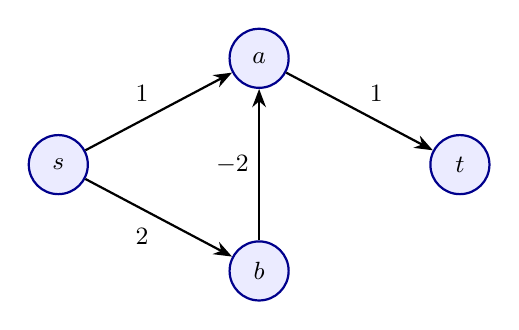
\begin{tikzpicture}[font=\small,>=Stealth,node distance=16mm]
  \node[vrch] (s) {$s$}; \node[vrch] (a) [above right=8mm and 20mm of s] {$a$};
  \node[vrch] (b) [below right=8mm and 20mm of s] {$b$}; \node[vrch] (t) [above right=8mm and 20mm of b] {$t$};
  \draw[sip] (s)--(a) node[midway,above left]{$1$};
  \draw[sip] (s)--(b) node[midway,below left]{$2$};
  \draw[sip] (b)--(a) node[midway,left]{$-2$};
  \draw[sip] (a)--(t) node[midway,above right]{$1$};
\end{tikzpicture}
\end{center}
\obrpopis{graf se zápornou hranou $b\!\to\!a$ ($-2$). Dijkstra uzavře $a$ s~$h(a)=1$ (přímou hranou $s\!\to\!a$) a~$t$ dostane $h(t)=2$. Levnější obchvat $s\!\to\!b\!\to\!a$ délky $2-2=0$ se objeví až po uzavření~$a$; verze, která uzavřené vrcholy nerelaxuje, vydá $d(s,t)=2$ místo správného $1$ (při obou pořadích uzavření $b$ a~$t$). Verze z~Průvodce $a$ znovu otevře a~$t$ opraví, zaplatí za to ale opakovaným zpracováním vrcholů. Bellman-Ford fázovou relaxací najde správně $d(s,a)=0$ a~$d(s,t)=1$ (přes $s\!\to\!b\!\to\!a\!\to\!t$). Záporných \emph{cyklů} zde není, vzdálenosti jsou dobře definované.}

\begin{priklad}[Simulace Dijkstrova algoritmu]
\textbf{Zadání.} Najděte Dijkstrovým algoritmem vzdálenosti z~$s$ v~grafu s~nezápornými hranami $s\!\to\!a\,(2)$, $s\!\to\!b\,(5)$, $a\!\to\!b\,(1)$, $a\!\to\!c\,(7)$, $b\!\to\!c\,(3)$, $b\!\to\!t\,(6)$, $c\!\to\!t\,(2)$.\par
\textbf{Řešení.} Vždy uzavřeme dosud neuzavřený vrchol s~nejmenším $h$ a~zrelaxujeme jeho hrany ($h(w)\leftarrow\min(h(w),\,h(v)+\ell(vw))$). Tabulka uzavírání:
\begin{itemize}
  \item Uzavři $s\,(h{=}0)$: relax $a\!\to\!2$, $b\!\to\!5$.
  \item Uzavři $a\,(h{=}2)$: relax $b\!\to\!\min(5,2{+}1){=}3$, $c\!\to\!2{+}7{=}9$.
  \item Uzavři $b\,(h{=}3)$: relax $c\!\to\!\min(9,3{+}3){=}6$, $t\!\to\!3{+}6{=}9$.
  \item Uzavři $c\,(h{=}6)$: relax $t\!\to\!\min(9,6{+}2){=}8$.
  \item Uzavři $t\,(h{=}8)$.
\end{itemize}
Výsledek $\boxed{d(s,\cdot)=(s{:}0,\,a{:}2,\,b{:}3,\,c{:}6,\,t{:}8)}$. Všimni si, že $c$ i~$t$ se po prvním nalezení ještě zlepšily (z~$9$ na $6$, resp.\ z~$9$ na~$8$) -- proto Dijkstra uzavírá až dosud nejmenší $h$, ne první nalezenou hodnotu.

\begin{center}
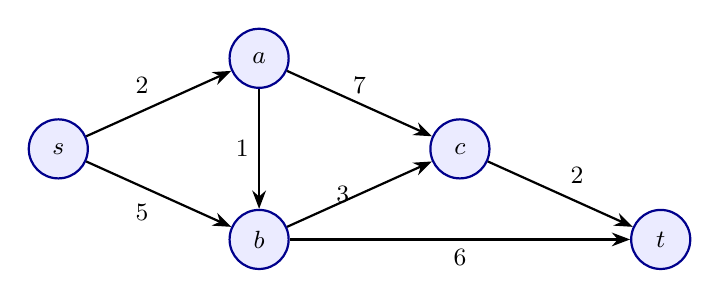
\begin{tikzpicture}[font=\small,>=Stealth,node distance=18mm]
  \node[vrch] (s) {$s$};
  \node[vrch] (a) [above right=6mm and 20mm of s] {$a$};
  \node[vrch] (b) [below right=6mm and 20mm of s] {$b$};
  \node[vrch] (c) [above right=6mm and 20mm of b] {$c$};
  \node[vrch] (t) [below right=6mm and 20mm of c] {$t$};
  \draw[sip] (s)--(a) node[midway,above left]{$2$};
  \draw[sip] (s)--(b) node[midway,below left]{$5$};
  \draw[sip] (a)--(b) node[midway,left]{$1$};
  \draw[sip] (a)--(c) node[midway,above]{$7$};
  \draw[sip] (b)--(c) node[midway,left]{$3$};
  \draw[sip] (b)--(t) node[midway,below]{$6$};
  \draw[sip] (c)--(t) node[midway,above right]{$2$};
\end{tikzpicture}
\end{center}
\end{priklad}

\subsection{Minimální kostra (Jarník, Borůvka)}

\begin{definice}[Kostra a minimální kostra]
\emph{Kostra} souvislého grafu $G$ je podgraf, který je strom a~obsahuje všechny vrcholy. \emph{Minimální kostra} (MST) je kostra s~nejmenším součtem vah hran. Mají-li hrany navzájem různé váhy, je MST určena jednoznačně.
\end{definice}

\begin{lemma}[Řezové lemma]
Nechť hrany mají navzájem různé váhy a~nechť $A\,\dot\cup\,B=V$ je rozdělení vrcholů na dvě neprázdné části. Pak \emph{nejlehčí hrana} vedoucí mezi $A$ a~$B$ leží v~každé minimální kostře.
\end{lemma}

\begin{proof}[Důkaz (výměnný argument).]
Nechť $e$ je nejlehčí hrana řezu mezi $A$ a~$B$ a~nechť nějaká kostra $T$ ji neobsahuje. Přidáním $e$ do $T$ vznikne cyklus, který řez překročí ještě v~nějaké jiné hraně $f$ (jdoucí mezi $A$ a~$B$). Protože $e$ je v~řezu nejlehčí a~váhy jsou různé, je $w(f)>w(e)$. Záměnou $T'=T-f+e$ dostaneme kostru s~menší vahou, takže $T$ nebyla minimální. Tedy každá MST obsahuje~$e$.
\end{proof}

\begin{center}
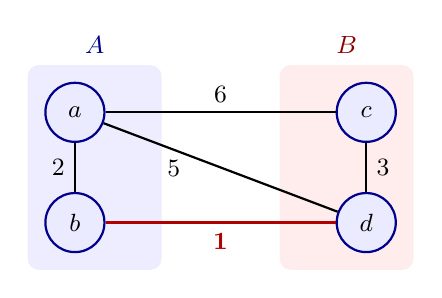
\begin{tikzpicture}[font=\small,node distance=14mm]
  \begin{scope}[on background layer]
    \fill[blue!7,rounded corners] (-0.6,-1.3) rectangle (1.1,1.3);
    \fill[red!7,rounded corners] (2.6,-1.3) rectangle (4.3,1.3);
  \end{scope}
  \node[vrch] (a1) at (0,0.7) {$a$}; \node[vrch] (a2) at (0,-0.7) {$b$};
  \node[vrch] (b1) at (3.7,0.7) {$c$}; \node[vrch] (b2) at (3.7,-0.7) {$d$};
  \draw[hrana] (a1)--(a2) node[midway,left]{$2$};
  \draw[hrana] (b1)--(b2) node[midway,right]{$3$};
  \draw[hrana,red!70!black,very thick] (a2)--(b2) node[midway,below]{$\mathbf 1$};
  \draw[hrana] (a1)--(b1) node[midway,above]{$6$};
  \draw[hrana] (a1)--(b2) node[pos=0.3,below]{$5$};
  \node[draw=none] at (0.25,1.55) {\textcolor{blue!55!black}{$A$}};
  \node[draw=none] at (3.45,1.55) {\textcolor{red!55!black}{$B$}};
\end{tikzpicture}
\end{center}
\obrpopis{řez mezi $A=\{a,b\}$ a~$B=\{c,d\}$. Hrany přes řez mají váhy $1,5,6$; nejlehčí ($b\!-\!d$, váha~$1$, zvýrazněná) podle řezového lemmatu leží v~každé MST. Toto lemma je společným základem korektnosti Jarníkova, Borůvkova i~Kruskalova algoritmu -- každý z~nich přidává hrany, které jsou nejlehčí v~nějakém řezu.}

\begin{veta}[Jarníkův a Borůvkův algoritmus]
Oba algoritmy najdou minimální kostru.
\begin{itemize}
  \item \textbf{Jarník:} pěstuje jeden strom od počátečního vrcholu; opakovaně přidá nejlehčí hranu vedoucí ze stromu ven. S~haldou běží v~čase $O(m\log n)$.
  \item \textbf{Borůvka:} začne lesem izolovaných vrcholů; v~každé \emph{fázi} přidá pro \emph{každou} komponentu její nejlehčí vnější hranu (všechny naráz). Počet komponent klesne aspoň na polovinu, takže fází je $\le\lceil\log_2 n\rceil$ a~celkový čas je $O(m\log n)$.
\end{itemize}
\end{veta}

\begin{intuice}
Korektnost obou plyne z~řezového lemmatu: Jarník bere nejlehčí hranu řezu „strom vs.\ zbytek``; Borůvka pro každou komponentu nejlehčí hranu řezu „komponenta vs.\ zbytek``. Obě tedy přidávají jen hrany, které musí být v~MST. (Příbuzný \textbf{Kruskalův} algoritmus třídí hrany podle váhy a~bere každou, která nespojí už spojené vrcholy; s~datovou strukturou Union-Find běží také $O(m\log n)$.)
\end{intuice}

\subsection{Toky v sítích (Ford--Fulkerson)}

\begin{definice}[Síť, tok, řez]
\emph{Síť} je orientovaný graf s~\emph{kapacitami} $c(e)\ge0$ na hranách a~dvěma vyznačenými vrcholy: \emph{zdrojem} $z$ a~\emph{stokem} $s$. \emph{Tok} je funkce $f(e)$ s~$0\le f(e)\le c(e)$ (kapacitní omezení), která v~každém vrcholu kromě $z,s$ splňuje \emph{zachování} (Kirchhoffův zákon): co přiteče, to odteče. \emph{Velikost toku} $|f|$ je čistý odtok ze zdroje. \emph{Řez} $(A,B)$ je rozdělení vrcholů s~$z\in A$, $s\in B$; jeho \emph{kapacita} je součet kapacit hran z~$A$ do~$B$.
\end{definice}

\begin{veta}[O maximálním toku a minimálním řezu]
Velikost maximálního toku se rovná kapacitě minimálního řezu (\emph{max-flow $=$ min-cut}). Fordův--Fulkersonův algoritmus maximální tok najde: dokud v~\emph{rezervní (reziduální) síti} existuje \emph{zlepšující cesta} ze $z$ do~$s$, pošle po ní co nejvíc toku.
\end{veta}

\begin{intuice}
Rezerva hrany je volná kapacita ve směru hrany plus možnost „vrátit`` už poslaný tok proti směru. Zlepšující cesta je cesta ze $z$ do~$s$ samými hranami s~kladnou rezervou; po ní přidáme tok o~velikosti minima rezerv na cestě. Když žádná taková cesta není, je tok maximální: množina $A$ vrcholů dosažitelných ze $z$ v~rezervní síti dává řez $(A,B)$, jehož hrany z~$A$ do~$B$ jsou nasycené a~hrany z~$B$ do~$A$ nevedou žádný tok, takže $|f|=c(A,B)$ -- a~protože $|f|\le c(\text{libovolný řez})$, je tento řez minimální a~tok maximální. (Pro celočíselné kapacity algoritmus skončí, každé zlepšení zvýší tok aspoň o~1.)
\end{intuice}

\begin{center}
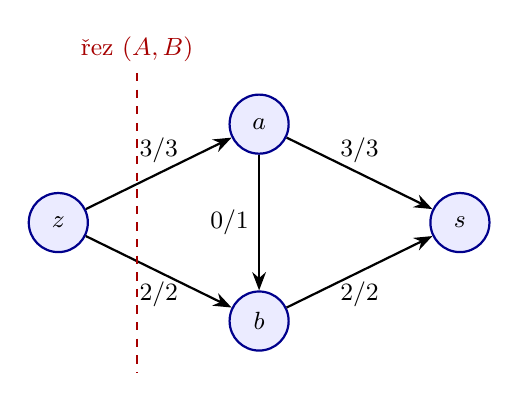
\begin{tikzpicture}[font=\small,>=Stealth,node distance=18mm]
  \node[vrch] (z) {$z$}; \node[vrch] (a) [above right=7mm and 20mm of z] {$a$};
  \node[vrch] (b) [below right=7mm and 20mm of z] {$b$}; \node[vrch] (s) [below right=7mm and 20mm of a] {$s$};
  \draw[sip] (z)--(a) node[midway,above]{$3/3$};
  \draw[sip] (z)--(b) node[midway,below]{$2/2$};
  \draw[sip] (a)--(b) node[midway,left]{$0/1$};
  \draw[sip] (a)--(s) node[midway,above]{$3/3$};
  \draw[sip] (b)--(s) node[midway,below]{$2/2$};
  \draw[dashed,red!65!black,thick] (1.0,1.9) -- (1.0,-1.9);
  \node[draw=none,red!65!black] at (1.0,2.2) {řez $(A,B)$};
\end{tikzpicture}
\end{center}
\obrpopis{síť s~popisky \emph{tok/kapacita}. Maximální tok má velikost $|f|=5$ (ze $z$ odtéká $3+2$). Minimální řez $A=\{z\}$, $B=\{a,b,s\}$ má kapacitu $c=3+2=5$. Rovnost $|f|=c(A,B)=5$ je věta max-flow $=$ min-cut; hrany řezu jsou nasycené ($3/3$, $2/2$), takže tok už nelze zvětšit.}

% ============================================================
\section*{Shrnutí}
\addcontentsline{toc}{section}{Shrnutí}

\begin{poznamka}
\textbf{Klíčové pojmy, fakta a~složitosti (přehled k~SZZ).} Stručný výčet klíčových pojmů, algoritmů a~jejich složitostí okruhu I2. Zkratky: $n$ = počet prvků / vrcholů, $m$ = počet hran.

\smallskip
\emph{Složitost algoritmů a~asymptotická notace.}
\begin{itemize}
  \item \textbf{Model RAM:} elementární operace (aritmetika, porovnání, přístup do paměti) každá $O(1)$; výsledky nezávisejí na HW až na konstantní faktor. Složitost v~\emph{nejhorším případě} = maximum přes vstupy velikosti $n$; \emph{nejlepší} = minimum; \emph{průměrný} = střední hodnota přes vstupy; bez poznámky myslíme nejhorší.
  \item $f\in O(g)$: $\exists c>0:\,f(n)\le c\,g(n)$ pro skoro všechna $n$ (horní odhad); $\Omega(g)$ -- dolní; $\Theta(g)$ -- těsný. Pravidla: v~součtu dominuje nejrychleji rostoucí člen; $\log n=O(n^\varepsilon)$ pro každé $\varepsilon>0$; $n^d=O(2^n)$.
  \item \textbf{Měření velikosti dat:} u~číselných úloh je velikost \emph{délka zápisu} (počet číslic/bitů), ne hodnota čísla. „Vyzkoušet dělitele do~$x$`` je $O(x)$, ale $x\approx 10^{\text{délka}}$, tedy \emph{exponenciální} v~délce zápisu (viz rozklad čísla).
\end{itemize}

\smallskip
\emph{Třídy složitosti P a~NP, NP-úplnost.}
\begin{itemize}
  \item $L\in\mathbf{P}$: $\exists$ algo.\ a~polynom $p$: pro každý $x$ doběhne v~$p(|x|)$ se správnou odpovědí. $L\in\mathbf{NP}$: $\exists$ verifikátor $K\in\mathbf{P}$ a~polynom $g$: $x\in L\Leftrightarrow\exists y,\,|y|\le g(|x|):\,K(x,y){=}1$ ($y$ = \emph{certifikát}; ověřit hotové řešení je v~P, najít ho nemusí být). Platí $\mathbf{P}\subseteq\mathbf{NP}$; zda $\mathbf{P}{=}\mathbf{NP}$, je otevřené.
  \item \textbf{Polynomiální převod} $A\le B$: $\exists$ polynomiálně spočitatelná $f$: $x\in A\Leftrightarrow f(x)\in B$. Obtížnost teče po šipce: $A\le B\wedge B\in\mathbf{P}\Rightarrow A\in\mathbf{P}$; obměna: $A\le B\wedge A\notin\mathbf{P}\Rightarrow B\notin\mathbf{P}$. Relace $\le$ je reflexivní a~tranzitivní.
  \item $L$ je \textbf{NP-těžký}: každý $M\in\mathbf{NP}$ se polynomiálně převede na~$L$. \textbf{NP-úplný} = NP-těžký $\wedge$ $L\in\mathbf{NP}$ (nejtěžší v~NP). Cook--Levinova věta (bez důkazu): \textsc{SAT} je NP-úplný.
  \item Klasické NP-úplné problémy: \textsc{SAT}, \textsc{3-SAT}, nezávislá množina, klika, $k$-barvení ($k\ge3$), Hamiltonovská kružnice, batoh, součet podmnožiny. Typický řetěz: $\textsc{SAT}\to\textsc{3-SAT}\to\text{nezáv.\ množina}\to\text{klika}$; $\textsc{3-SAT}\to\text{3-barvení}$.
  \item Postup NP-úplnosti nového $M$: (1) $M\in\mathbf{NP}$ -- popsat certifikát a~polynomiální verifikátor; (2) $L\le M$ pro nějaký NP-úplný $L$ -- zkonstruovat polynomiální převod $f$.
\end{itemize}

\smallskip
\emph{Metoda rozděl a~panuj, Master theorem.}
\begin{itemize}
  \item Rekurence: $T(n)=a\,T(n/b)+\Theta(n^c)$, $T(1)=\Theta(1)$.
  \item \textbf{Master theorem} (bez důkazu): nechť $q=a/b^c$:
    $q<1\;\Rightarrow\;T(n)=\Theta(n^c)$ (dominuje kořen stromu rekurze);
    $q=1\;\Rightarrow\;T(n)=\Theta(n^c\log n)$ (všechny hladiny stejné);
    $q>1\;\Rightarrow\;T(n)=\Theta(n^{\log_b a})$ (dominují listy).
  \item Příklady: Mergesort $a{=}b{=}2,c{=}1$: $q{=}1\Rightarrow\Theta(n\log n)$; Karacuba $a{=}3,b{=}2,c{=}1$: $q{=}3/2{>}1\Rightarrow\Theta(n^{\log_2 3})\approx\Theta(n^{1{,}585})$; medián 2~polí $a{=}1,b{=}2,c{=}0$: $q{=}1\Rightarrow\Theta(\log n)$.
  \item \textbf{Mergesort:} dělí na~2 poloviny, slévá $\Theta(n)$; vždy $\Theta(n\log n)$; stabilní; prostor $\Theta(n)$. Slévání $k$ posloupností s~celkem $n$ prvky přes haldu: $\Theta(n\log k)$ (každý prvek jednou do/z haldy velikosti $k$).
  \item \textbf{$k$-tý nejmenší prvek:} Quickselect (jedna rekurze podle pivota) má s~náhodným pivotem očekávaný čas $\Theta(n)$; LinearSelect (medián mediánů pětic jako pivot) zaručí části zhruba $\le\tfrac{7}{10}n$, $T(n)=T(n/5)+T(7n/10)+\Theta(n)=\Theta(n)$ v~nejhorším případě.
\end{itemize}

\smallskip
\emph{Binární vyhledávací stromy (BST, AVL) a~halda.}
\begin{itemize}
  \item \textbf{BST -- uspořádací vlastnost:} $\text{levý podstrom}<k(v)<\text{pravý podstrom}$ v~každém vrcholu. Operace \textsc{Find}/\textsc{Insert}/\textsc{Delete} v~$\Theta(h)$; in-order průchod vydá vzestupně setříděný výpis.
  \item \textbf{Následník} (nejmenší klíč ostře větší než~$x$): má-li vrchol pravý podstrom, jdi do jeho nejlevějšího vrcholu; jinak stoupej nahoru, dokud nejsi levým synem -- ten otec je následník. Složitost $\Theta(h)$.
  \item Degenerace (liána): setříděné vstupy $\Rightarrow h=\Theta(n)\Rightarrow$ operace $\Theta(n)$. Porovnávání klíčů délky $L$ (řetězce) násobí cenu faktorem $L$: třídění $n$ řetězců AVL stromem = $O(n\cdot L\cdot\log n)$.
  \item \textbf{AVL strom:} BST s~podmínkou $|h(\ell)-h(r)|\le1$ v~každém vrcholu ($h$ = hloubka podstromu). Dolní mez: nejřidší AVL strom splňuje $A_h=A_{h-1}+A_{h-2}+1$, $A_0=1$, $A_1=2$, tedy $A_h\ge\varphi^h$ -- odkud $n\ge\varphi^h$, tj.\ $h=O(\log n)$. Operace $\Theta(\log n)$ s~$O(\log n)$ rotacemi. Třídění přes AVL (vložení $+$ in-order): $\Theta(n\log n)$; z~dolního odhadu třídění $\Omega(n\log n)$ plyne dolní mez $\Omega(\log n)$ na BST operace.
  \item \textbf{Binární halda:} úplný bin.\ strom uložený v~poli, haldová podmínka (kořen = globální minimum). \textsc{Insert} a~\textsc{ExtractMin} $O(\log n)$; \textsc{Min} $O(1)$. Využití: Dijkstra, Jarník, slévání $k$ posloupností.
\end{itemize}

\smallskip
\emph{Třídění.}
\begin{itemize}
  \item \textbf{Primitivní ($\Theta(n^2)$):} Selectsort -- vždy $\Theta(n^2)$, nestabilní; Insertsort -- nejlepší $\Theta(n)$ (téměř setříděný vstup), stabilní; Bubblesort -- nejlepší $\Theta(n)$ (detekcí průchodu beze změny), stabilní.
  \item \textbf{Quicksort:} průměrný $\Theta(n\log n)$, nejhorší $\Theta(n^2)$ (pivot = min/max, nastane např.\ setříděný vstup s~pivotem na kraji); nestabilní; prostor $O(\log n)$ na zásobník (rekurze nejdřív do menší části). Náhodná volba pivota $\Rightarrow\Theta(n\log n)$ v~očekávání.
  \item \textbf{Mergesort:} vždy $\Theta(n\log n)$, stabilní, prostor $\Theta(n)$ (viz rozděl a~panuj).
  \item \textbf{Dolní odhad} porovnávacího třídění: $\Omega(n\log n)$ v~nejhorším případě. Argument: rozhodovací strom má $\ge n!$ listů (různá pořadí $\Rightarrow$ různé listy); hloubka $\ge\log_3(n!)=\Theta(n\log n)$ (z~$n!\ge(n/2)^{n/2}$).
  \item \textbf{Inverze} = dvojice $(i<j)$ s~$a_i>a_j$; Insertsort a~Bubblesort prohazují jen sousedy, tj.\ opraví jednu inverzi na krok, takže $\Omega(n^2)$ na obrácené posloupnosti (Selectsort je $\Theta(n^2)$ kvůli porovnáním). \textbf{Stabilní} algoritmus zachovává pořadí prvků se stejným klíčem.
\end{itemize}

\smallskip
\emph{Grafové algoritmy.}
\begin{itemize}
  \item \textbf{Reprezentace:} matice sousednosti $\Theta(n^2)$, hrana $O(1)$; seznamy sousedů $\Theta(n+m)$, iterace sousedů rychlá; pro řídké grafy volíme seznamy.
  \item \textbf{BFS} $\Theta(n+m)$: fronta, vrstvy, vzdálenosti v~počtu hran. \textbf{DFS} $\Theta(n+m)$: zásobník/rekurze, časy $\mathrm{in}/\mathrm{out}$ (závorkování). \textbf{Topologické třídění} DAGu: DFS + klesající $\mathrm{out}(v)$ (nebo odebírání zdrojů); $\Theta(n+m)$; existuje $\Leftrightarrow$ DAG.
  \item \textbf{Dijkstrův algoritmus:} nezáporné délky hran; relaxace v~pořadí rostoucí $h$ (halda); $O((n+m)\log n)$. Při záporné hraně invariant (uzavřený $\Rightarrow$ správná vzdálenost) selže.
  \item \textbf{Bellmanův--Fordův algoritmus:} záporné hrany povoleny, bez záporných cyklů; $n-1$ fází -- v~každé zrelaxuj všechny hrany; $O(nm)$. Záporný cyklus $\Leftrightarrow$ $n$-tá fáze stále mění~$h$.
  \item \textbf{Minimální kostra} (MST) -- \emph{řezové lemma}: světlá (nejlehčí) hrana přes libovolný řez leží v~každé MST. Jarník (Prim): z~jednoho vrcholu hladově s~haldou, $O(m\log n)$. Borůvka: paralelní přidávání nejlehčí vnější hrany každé komponenty, $\lceil\log_2 n\rceil$ fází, $O(m\log n)$. Kruskal: setřídit hrany + Union-Find, přidávat nejlehčí nespojující tutéž komponentu, $O(m\log n)$.
  \item \textbf{Toky v sítích:} tok $f$ splňuje $0\le f(e)\le c(e)$ (kapacita) a~Kirchhoffův zákon. Ford--Fulkerson augmentuje po nenasycených cestách v~reziduální síti; pro celočíselné kapacity terminuje. \textbf{Věta max-flow $=$ min-cut}: velikost max.\ toku $=$ kapacita min.\ řezu.
\end{itemize}
\end{poznamka}

\section*{Zdroje}
\addcontentsline{toc}{section}{Zdroje}

{\raggedright
\begin{itemize}
  \item M.~Mareš, T.~Valla: \emph{Průvodce labyrintem algoritmů}, 2.~vydání, edice CZ.NIC, Praha 2022 (doporučená učebnice předmětů NTIN060 a~NTIN061, jediný primární zdroj výkladu; licence CC BY-ND 4.0, volně ke stažení).\\ \url{https://pruvodce.ucw.cz/}
  \item MFF UK: požadavky ke státní závěrečné zkoušce (Informatika, Bc.) a~zadání otázek z~minulých termínů.\\ \url{https://www.mff.cuni.cz/cs/studenti/bakalarske-studium/statni-zaverecne-zkousky/bakalarske-statni-zkousky-studijniho-programu-informatika}
\end{itemize}
\par}

\end{document}
